 % TO DELETE

%    \documentclass[journal,a4paper]{IEEEtran}
%  \documentclass[journal]{IEEEtran}

%      \documentclass[10pt,twocolumn,twoside]{IEEEtran}
     \documentclass[11pt,draftcls,onecolumn,peerreview]{IEEEtran} 
%         \topmargin       -6.0mm
%          \oddsidemargin      0mm
%          \evensidemargin     0mm
%          \textheight     223.5mm
%         \textwidth      170.0mm
\usepackage{setspace} 
\usepackage{color}
\newcommand{\mike}[1]{\textcolor{red}{#1}}
\newcommand{\dean}[1]{\textcolor{green}{#1}}
\newcommand{\parham}[1]{\textcolor{blue}{#1}} 
\newcommand{\ken}[1]{\textsf{\emph{\textbf{\textcolor{magenta}{#1}}}}} 
\newcommand{\cut}[1]{\textcolor{cyan}{#1}} 

\usepackage{cite}
%Reduce the spacing between figures and captions
% \usepackage[belowskip=-15pt,aboveskip=10pt]{caption}
%  \setlength{\intextsep}{2pt plus 2pt minus 2pt}

\ifCLASSINFOpdf
   \usepackage[pdftex]{graphicx}
  % declare the path(s) where your graphic files are
  % \graphicspath{{../pdf/}{../jpeg/}}
  % and their extensions so you won't have to specify these with
  % every instance of \includegraphics
  % \DeclareGraphicsExtensions{.pdf,.jpeg,.png}
\else
  % or other class option (dvipsone, dvipdf, if not using dvips). graphicx
  % will default to the driver specified in the system graphics.cfg if no
  % driver is specified.
  \usepackage[dvips]{graphicx}
  % declare the path(s) where your graphic files are
  % \graphicspath{{../eps/}}
  % and their extensions so you won't have to specify these with
  % every instance of \includegraphics
  % \DeclareGraphicsExtensions{.eps}
\fi

\usepackage[cmex10]{amsmath}
\interdisplaylinepenalty=2500
\usepackage{amssymb}
\ifCLASSOPTIONcompsoc
  \usepackage[tight,normalsize,sf,SF]{subfigure}
\else
  \usepackage[tight,footnotesize]{subfigure}
\fi

\usepackage{natbib}

\usepackage{stfloats}
\usepackage{float}
\floatstyle{ruled}
%This bit is how to use hyperlink without stupid coloured rectangles around it
\usepackage{float}
\usepackage{hyperref}
\hypersetup{colorlinks,linkcolor=black,filecolor=black,urlcolor=black,citecolor=black}
%~~~~~~~~~~~~~~~~~~~~~~~~~~~~~~~~~~~~~~~~~
\newfloat{algorithm}{htbp}{loa}%[chapter]
\floatname{algorithm}{Algorithm}

\begin{document}
%
% paper title
% can use linebreaks \\ within to get better formatting as desired
\title{Spatiotemporal Multi-Resolution Approximation of the Amari Type Neural Field Model}


\author{P. Aram, D.R. Freestone~\IEEEmembership{Graduate Student Member,~IEEE}, M. Dewar, K.Scerri~\IEEEmembership{Member,~IEEE}, D.B. Grayden~\IEEEmembership{Member,~IEEE,} and V. Kadirkamanathan~\IEEEmembership{Member,~IEEE} % <-this % stops a space
\thanks{P. Aram* and V. Kadirkamanathan are with the Department of Automatic Control and Systems Engineering, University of Sheffield, Sheffield, S1 3JD, U.K. (e-mail:parham.aram@univ-amu.fr; visakan@sheffield.ac.uk).}% <-this % stops a space
\thanks{D.\ R.\ Freestone and D.\ B.\ Grayden are with the Department
of Electrical and Electronic Engineering, The University of Melbourne, and The Bionic Ear Institute, VIC, Australia. (e-mail:dfreestone@bionicear.org; grayden@unimelb.edu.au). The Bionic Ear Institute acknowledges the support it receives from the Victorian State Government through the Operational Infrastructure Support Program.}
\thanks{M. Dewar is with the Department of Applied Physics and Applied Mathematics, Columbia University, New York, NY, USA. (e-mail:mike.dewar@columbia.edu).}
\thanks{K. Scerri is with the Department of Systems and Control Engineering, University
of Malta, Msida, MSD, Malta. (e-mail:kenneth.scerri@um.edu.mt).}}
% <-this % stops a space
%\thanks{Manuscript received April 19, 2005; revised January 11, 2007.}}



% The paper headers
% \markboth{Journal of }%
% {Aram \MakeLowercase{\textit{et al.}}: Wavelet Multiresolution Spatio-Temporal Modelling Using the Integro-Difference Equation}
% The only time the second header will appear is for the odd numbered pages
% after the title page when using the twoside option.
% 
% *** Note that you probably will NOT want to include the author's ***
% *** name in the headers of peer review papers.                   ***
% You can use \ifCLASSOPTIONpeerreview for conditional compilation here if
% you desire.
 \ifCLASSOPTIONpeerreview
\else
\fi

% If you want to put a publisher's ID mark on the page you can do it like
% this:
%\IEEEpubid{0000--0000/00\$00.00~\copyright~2007 IEEE}
% Remember, if you use this you must call \IEEEpubidadjcol in the second
% column for its text to clear the IEEEpubid mark.

% make the title area
\maketitle


\begin{abstract}
%\boldmath
We develop a multi-resolution approximation (MRA) framework for the integro-difference equation (IDE) neural field model based on semi-orthogonal cardinal B-spline wavelets. State and parameter estimation is performed using the Expectation Maximization (EM) algorithm. A synthetic example is provided
to demonstrate the framework.
\end{abstract}
% Note that keywords are not normally used for peerreview papers.
 \begin{IEEEkeywords}
  Neural field model, multi-resolution approximation (MRA), Expectation Maximization (EM) algorithm, wavelets.
  \end{IEEEkeywords}
% For peer review papers, you can put extra information on the cover
% page as needed:
% \ifCLASSOPTIONpeerreview
%   \begin{center} \bfseries EDICS Category: SSP-IDEN \end{center}
%   \fi
%
%  For peerreview papers, this IEEEtran command inserts a page break and
%creates the second title. It will be ignored for other modes.
\IEEEpeerreviewmaketitle


\section{Introduction}
\IEEEPARstart{T}{he} human cerebral cortex has a multi-resolution architecture, where spatial scales for information processing range from ion channels, to single neurons, to networks of millions of neurons. This multi-resolution cortical architecture poses major modeling challenges to efficiently describe the brain's dynamics. This paper introduces a multi-resolution data-driven framework for neural field modeling, the Multi-Resolution Approximate Integro-Difference Equation (MRAIDE), to address this challenge. 

Neural field models describe the mass action of the central nervous system and are a critical link in our understanding of the biophysics of the EEG. The key components of these models typically describe the macroscopic dynamics of the human brain, but can also descriptive of finer-scale neurodynamics. \parham{Examples are, the post-synaptic response kernels (the pulse to wave function) and the activation function (wave to pulse function) \citep{Jirsa1997}. The former can be descriptive of inhibitory and excitatory post-synaptic potentials in microscopic single neural models, such as integrate and fire, or an ensemble response to stimulation in macroscopic neural mass models. The latter,  can be used to model spiking statistics across spatial scales from single neurons (where it can be considered a CDF of the probability of firing) to mean firing rates of neural masses.} The key factor linking the key functions of the model to particular spatial scales is geometry of the connectivity, hence the ability to infer a multi-resolution connectivity kernel will enable to the formulation of a multi-resolution neural field model. 

The utility of these models for answering questions in clinical neuroscience and neurology lies in the ability to infer parameters from electrophysiological data. The ability to create patient-specific neural models will contribute to our knowledge base of diseases such as epilepsy and will enable the development of new treatment strategies. This is particularly relevant to the advent of new devices that use therapeutic electrical stimulation. Stimulation strategies for devices currently operate in an open loop, where stimulation parameters are chosen using a process of trial and error. Therefore, there exists enormous potential to improve the performance of these devices using systems theory, which in turn requires a suitable dynamic model. Neural mass and neural field models are ideal candidates for estimation algorithms due to their strong links with physiology and their parsimony. It is expected that parameters of the neural fields models will be patient-specific and will, therefore, need to be inferred from data.

The first work (to the authors best knowledge) describing data-driven mesoscopic neural modelling used a neural mass model to fit EEG data~\citep{Valdes1999}. This approach was extended to coupled neural masses through a Bayesian estimation scheme dubbed Dynamic Causal Modelling (DCM)~\citep{David2003}. Following this work, data-driven modelling was extended to continuum field equations that explained the richer dynamics of spatiotemporal neural fields \citep{Galka2008,schiff2008kalman,Daunizeau2009}. Most recently, a framework was developed where a finite element model (FEM) of the neural field (via a global Galerkin projection) was formed, using a basis function decomposition, to transform the PDE neural field equations into a finite dimension system to facilitate efficient state and parameter estimation~\citep{Freestone2011}. This paper is an extension to the aforementioned study, where we derive a neural field state-space model that accounts for the multi-resolution architecture and spatial dynamics of the human cortex. In this way, a flexible framework is created, whereby both macroscopic and microscopic behaviour of the system can be represented simultaneously and completely.

\section{Multi-Resolution Cortical Architecture}
The human neocortex has an inherent multi-resolution architecture. The spatiotemporal neural field can be written as 
\begin{equation}
	v\left(\mathbf{r},t\right) = \sum_{j} v_j\left(\mathbf{r},t\right),
\end{equation}
where $v\left(\mathbf{r},t\right)$ is a voltage field that may be measured with a multi-electrode array or voltage sensitive dye, $\mathbf{r}\in \mathbb{R}^n$ (where $n\le3$) describes the spatial location within the field, $t$ denotes time, and $j$ indexes the different levels of resolution in the field. This multi-resolution structure is depicted in Figure~\ref{fig:MultiLayerFieldModel}.
\begin{figure}[t]
	\centering
		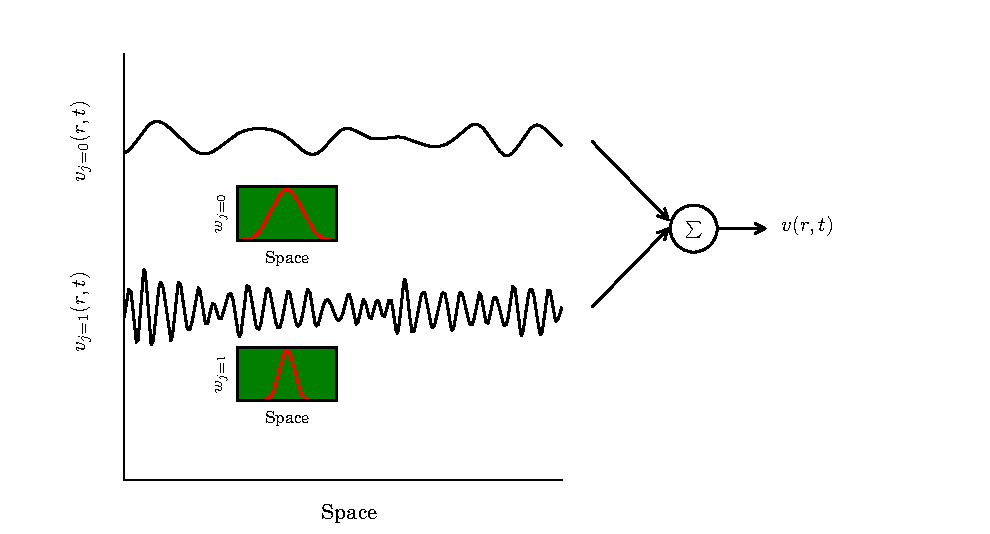
\includegraphics[scale=1]{./Graph/MultiResNeuralField.pdf}
	\caption{{\bf Multi-layer neural field model}. The inset figures show the shape of the
connectivity kernel components at each spatial resolution.}
	\label{fig:MultiLayerFieldModel}
\end{figure}

The multi-resolution structure has been described by numerous methods. For example, this idea of multi-resolution can be thought of a generalisation of modelling the layers of the cortex separately, where the connectivity kernel, or neural foot-print, has varying widths \citep{Wilson1973}.

Typically, the experimentalist only has access the net field generated by the multi-resolution architecture. Follow this, it is natural to ask how do we best describe the multi-resolution structure of the neural system. The solution to this problem was proposed by \citet{Breakspear2005} in using a wavelet decomposition. This paper is directed at developing a framework for patient-specific multi-resolution neural field models. 

\section{IDE Neural Field Model}
\singlespacing
\begin{table*}[!t]
\begin{tabular}{|l|l|l|}
	\hline
	\textbf{Symbol} & \textbf{Quantity} & \textbf{Units}\\
	\hline
	\multicolumn{3}{|c|}{\emph{Domain and indices}}\\
	\hline
	$\Omega$ & spatial domain & n.a.\\
	$\mathbf{r}$ & spatial location & [mm, mm]\\
	$t$ & time & s\\
	\hline
	\multicolumn{3}{|c|}{\emph{Model}}\\
	\hline
    $y_t$ & observation & mV\\
    $v(\mathbf{r},t)$ & mean membrane potential & mV \\
	$f(v\left(\mathbf{r},t\right))$ & firing rate function & spikes.s$^{-1}$\\
	$e(\mathbf{r},t)$ & field disturbance, with covariance function $\gamma(\mathbf r-\mathbf r')$ & mV\\
	$\boldsymbol\varepsilon_t$ & observation noise, with covariance matrix $\Sigma_\varepsilon$ & mV\\
	$m(\mathbf{r}_n)$ & observation kernel where $n$ is sensor index $n=1,..,n_y$ (width $\sigma_m$) & n.a. \\
	$w(\mathbf{r})$ & spatial connectivity kernel & n.a.\\
	$h(t)$ & post-synaptic response kernel & mV\\
	$\zeta$, $\xi$ & inverse synaptic time constant \& time constant parameter & s$^{-1}$, n.a.\\
	$\eta(t)$ & Heaviside step function & n.a.\\
	$\delta(t)$ & Dirac-delta function & n.a.\\
	$\textrm{D}$ & temporal differential operator & n.a.\\
	\hline
	\multicolumn{3}{|c|}{\emph{Reduced Model}} \\
	\hline
   	$\mathbf{x}_t$ & state vector at time $t$ & mV\\
   	$\mathbf{e}_t$ & state disturbance vector, with covariance $\Sigma_e$ & mV\\
   	$\mathbf{C}$ & observation matrix & n.a. \\
	\hline
	\multicolumn{3}{|c|}{\emph{Frequency Analysis}} \\
	\hline
	$\boldsymbol{\nu}$, $\boldsymbol{\nu}_c$ & spatial frequency and spatial cutoff frequency & cycles/mm \\
	$\sigma_{\nu}^2$ & variance of Fourier transformed Gaussian basis function & (cycles/mm)$^2$\\
	\hline
	\multicolumn{3}{|c|}{\emph{Estimation}} \\
	\hline
	$\mathcal K_{t} $ & filter gain & n.a.\\
	\hline
\end{tabular}
\caption{\textbf{Notation.} The first column of the table gives the symbols for all the notation used in the paper. The second column provides a brief description of the quantity, and the third column provides the SI units where relevant.}
\label{tab:Notation}
\end{table*}
\doublespacing

The single layer homogeneous neural field model in the most general form is described by the equation
\begin{equation}
	\label{FullDoubleIntModel} \underbrace{v\left(\mathbf{r},t\right)}_{\text{field}} =
	\int_{-\infty}^t 
	\underbrace{h\left(t - t'\right)}_{\text{synapse}} \int_\Omega
	\theta\underbrace{w\left(\mathbf{r},\mathbf{r}'\right)}_{\text{connectivity}} 
	\underbrace{f\left( v\left( \mathbf{r}',t' \right)\right)}_{\text{firing}}
	\, \mathrm{d}\mathbf{r}'\mathrm{d}t',
\end{equation}
where the post-synaptic membrane voltage at time $t$ of a population of neurons at position $\mathbf r$ within the spatial domain $\Omega$ is denoted by $v\left(\mathbf r,t\right)$. The function $h(t)$ describes the post-synaptic response kernel, $w(\mathbf{r})$ describes the connectivity kernel and $f(v(\mathbf{r},t))$ describes the relationship between the mean membrane potential and the mean firing rate. The parameter $\theta$ can be thought of the synaptic efficiency or coupling strength, where $\theta>0$ and $\theta<0$ describes excitation and inhibition, respectively. There are various forms of $h(t)$ that have been proposed in the literature, with different levels of complexity. These are shown in Figure~\ref{fig:Modelcomponents}. Similarly, both the connectivity kernel and the activity function (firing rate) can take various forms. These are also shown in Figure~\ref{fig:Modelcomponents}. The form of $w(\mathbf{r})$ typically describes an Laplacian (exponential) or Gaussian decay in connectivity strength from any point in the field. By assuming the form of $h(t)$ is the same across layers (scales) the Amari style neural field model is formed, incorporating a multilayer structure into the connectivity kernel. In this way, the connectivity kernel typically takes the form of a Mexican hat (Gaussian shape within layer connectivity) or Wizard hat (Laplacian shape within layer) as depicted in Figure~\ref{fig:Modelcomponents}.

The stochastic IDE form of the Amari neural field formulation~\cite{Amari1977} is given by (see~\cite{Freestone2011} for a full derivation)
\begin{equation}\label{eq:DiscreteTimeModel}
	v_{t+1}\left(\mathbf{r}\right) = 
	\xi v_t\left(\mathbf{r}\right) + 
	T_s \int_\Omega { 
	    w\left(\mathbf{r},\mathbf{r'}\right)
	    f\left(v_t\left(\mathbf{r}'\right)\right) 
	\, \mathrm{d}\mathbf{r}'} 
	+ e_t\left(\mathbf{r}\right), 
\end{equation}
where in this first-order (in time) form of the model the membrane dynamics are included through the parameter $\xi=1-T_s/\tau$, where $\tau$ is the membrane time constant and $T_s$ is the sampling time. 
% The connectivity strength between neural populations at a distance $\mid\mathbf{r}-\mathbf{r'}\mid$ is described by the connectivity kernel $w\left(\mathbf{r}-\mathbf{r}'\right)$. The connectivity kernel is taken as a ``Mexican hat'' function, which describes local excitation and lateral inhibition \cite{Amari1977,Atay2005}. The components of the model are shown in Figure~\ref{fig:Modelcomponents}
\begin{figure}[!t]
\centering
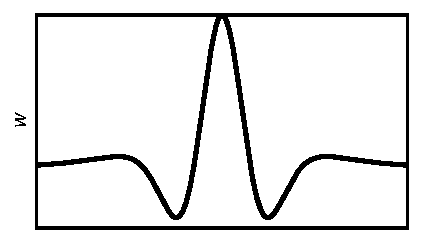
\includegraphics[scale=.6]{./Graph/ConnectivityKernel.pdf}
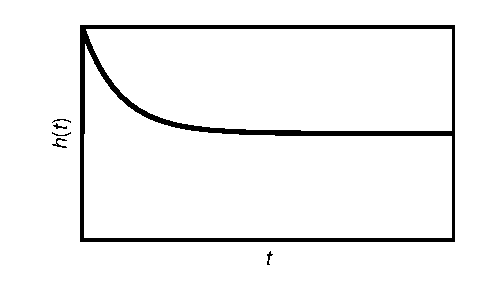
\includegraphics[scale=.6]{./Graph/Synaptickernel.pdf}
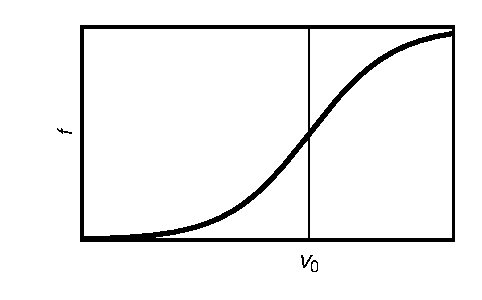
\includegraphics[scale=.6]{./Graph/Sigmoid.pdf}
\caption{ {\bf The IDE neural field model components}. (\textbf{a}) The mexican hat connectivity kernel. (\textbf{b}) First order synaptic kernel. (\textbf{c}) A representative of the activation function.}
\label{fig:Modelcomponents}
\end{figure}

The term $e_t(\mathbf r)$ is a zero mean Gaussian disturbance, spatially coloured but temporally white, with covariance function 
\begin{equation}
cov\left(e_{t}\left(\mathbf{r}\right),e_{t+t'}\left(\mathbf{r'}\right)\right)=\eta(\mathbf{r}-\mathbf{r'})\delta(t-t'),
\label{eq:FieldDisturbance}
\end{equation}
where $\delta(\cdot)$ is the Dirac-delta function. The firing rate of the presynaptic neurons is related to the post-synaptic membrane potential by the activation function $f(v_t(\mathbf{r}))$ \parham{Dean: can you add the bit about different type of activatin functions here}.%$ = \varsigma v_t(\mathbf{r})$ \cite{VanRotterdam1982,Murphy2009}.

The observation equation describing the intracranial electrophysiological recordings is given by
\begin{equation}\label{eq:ObservationEquation}
	y_t(\mathbf{r}_{n_y}) = \int_{\Omega} { m\left(\mathbf{r}_{n_y}-\mathbf{r}'\right) v_t\left(\mathbf{r}'\right) \, \mathrm{d}\mathbf{r}'} + \boldsymbol\epsilon_t(\mathbf{r}_{n_y}), 
\end{equation}
where $m\left(\mathbf{r}_{n_y}-\mathbf{r}'\right)$ is the observation kernel at location $\mathbf{r}_{n_y}$ and  $\boldsymbol{\epsilon}_{t}\sim \mathcal{N}\left(\mathbf{0},\mathbf{\Sigma}_{\epsilon}\right)$  is an i.i.d. Gaussian white noise process and the covariance matrix $\mathbf{\Sigma}_{\epsilon}=\sigma^2_{\epsilon}\mathbf I_{n_y}$, where $\mathbf I$ denotes the identity matrix. \parham{the lead field thingy} 

\section{MRA of the IDE in State-Space}
The purpose of forming the multi-resolution approximation (MRA) of the integro-difference equation (IDE) is to form a multi-resolution finite-dimensional state-space model that best captures the spatiotemporal characteristics of the neural field. Given such a model, it is then possible to perform state and parameter estimation in an efficient and robust manner, thus allowing for subject-specific models.

The goal of this section is to demonstrate how to formulate a state-space model in a canonical form such that standard algorithms may be applied to estimate the multi-resolution connectivity structure. Therefore, the goal is to form a parameterised equation for coefficients of the field basis functions $\mathbf{x}_t$, which becomes the state vector.

The multi-resolution approximation \citep{Mallat1989a} of the neural IDE (MRAIDE) is obtained by decomposing both the field, $v_t(\cdot)$, and the connectivity kernel, $w(\cdot)$, (assuming square-integrable functions) using translations and dilations of a scaling function $\phi(\mathbf{r})$ and a mother wavelet $\psi(\mathbf{r})$. Considering a  one-dimensional field, the static connectivity kernel is decomposed as,
\begin{equation}
 w\left(r\right)=\sum_{l\in \mathbb{Z}}\alpha_{j_0,l} \underbrace{\phi_{j_0,l}\left(r\right)}_{\text{scaling}} + \sum_{j\geq j_0}^{\infty} \sum_{l \in \mathbb{Z}}\beta_{j,l} \underbrace{\psi_{j,l}\left(r\right)}_{\text{wavelet}}, 
\label{eq:KernelExpansion}
\end{equation}
where $\alpha_{j_0,l}$ are the approximation coefficients at the lowest scale $j_0$, and $\beta_{j,l}$ are the detail coefficients at different scales $j$, with
\begin{align}
\phi_{j,l}\left(r\right) =& 2^{\frac{j}{2}}\phi\left(2^j r-l\right) \\	
\psi_{j,l}\left(r\right) =& 2^{\frac{j}{2}}\psi\left(2^j r-l\right).
\end{align}
The parameters $j$ and $l$ control the scale (dilation) and translation (spatial shift), respectively. \dean{NEED SOMETHING ABOUT HOW j AND l ARE SET HERE - AS IN THAT THEY ARE KNOWN - AND THAT WE ONLY NEED TO ESTIMATE THE COEFFICIENTS.} \parham{The number of spatial shifts is dependent on the scale, $j$, and can be chosen such that the basis functions cover the spatial domain. The number of scales depends on the spectral characteristics of the field, which will be described later.} Scaling functions retain the lowest frequency components, due to their low-pass properties, while the wavelet functions extract successively higher frequency components due to their band-pass characteristics. 

% At each spatial scale indexed by $j$ (level of decomposition), the neural field can be written as
% \begin{equation}
% 	v_{j,t}\left(\mathbf{r}\right) = \begin{cases}
% 	\sum_{l \in \mathbb{Z}}x_{j,l}(t) \underbrace{\phi_{j,l}\left(\mathbf{r}\right)}_{\text{scaling function}} + \check{x}_{t,j,l}\underbrace{\psi_{j,l}\left(\mathbf{r}\right)}_{\text{mother wavelet}} & \text{if $j=0$},\\
% 	\sum_{l \in \mathbb{Z}}\check{x}_{t,j,l}\psi_{j,l}\left(\mathbf{r}\right) & \text{otherwise}
% \end{cases}
% \end{equation}

The dynamic neural field is decomposed using
\begin{equation}
 v_t\left(r\right)=\sum_{l \in \mathbb{Z}}x_{t,j_{0},l} \underbrace{\phi_{j_0,l}\left(r\right)}_{\text{scaling}} + \sum_{j\geq j_0}^{\infty} \sum_{l \in \mathbb{Z}^n} \check{x}_{t,j,l} \underbrace{\psi_{j,l}\left(r\right)}_{\text{wavelet}},
\label{eq:FieldExpansion}
\end{equation}
where $x_{t,j_{0},l}$ and $\check{x}_{t,j,l} $ are the dynamic coefficients of the expansion, constituting the state vector at time $t$. \dean{The decomposition enables a separation of the static spatial characteristics, which are considered static functions, that are weighted by dynamic coefficients.}

Equations \ref{eq:KernelExpansion} and \ref{eq:FieldExpansion} are infinite series expansions and must be truncated to some level \dean{$j=J$} in order to solve the estimation problem. In other words, the neural field must be band-limited up to a given spatial frequency. 

Now we will simplify the notation by defining vectors that contain all the translations of the wavelets and scaling functions \parham{and their corresponding coefficients such that}
\begin{align}      
	\boldsymbol\phi_{j_0}(r) \triangleq&\left\lbrace{\phi_{j_0,l}(r)}:l \in \mathbb{Z} \right\rbrace \\
	\boldsymbol\psi_{j}(r) \triangleq& \left\lbrace{\psi_{j,l}(r)}:l \in \mathbb{Z} \right\rbrace\\
	\boldsymbol\alpha_{j_0} \triangleq& \left\lbrace\alpha_{j_0, l}:l \in \mathbb{Z} \right\rbrace \\
	\boldsymbol\beta_{j} \triangleq& \left\lbrace\beta_{j, l}:l \in \mathbb{Z} \right\rbrace \\
	\mathbf{x}_{t,j_0} \triangleq& \left\lbrace{x}_{t,j_{0},l}:l \in \mathbb{Z} \right\rbrace \\
	\check{\mathbf{x}}_{t,j} \triangleq& \left\lbrace{\check{x}}_{t,j,l}:l \in \mathbb{Z} \right\rbrace,
\end{align}
where $k = j_0,j$. Following this we can define the \dean{vectors} 
\begin{align}
\boldsymbol\theta^\top \triangleq& [\begin{array}{ccccc} \boldsymbol\alpha_{j_0}^\top & \boldsymbol\beta_{j_0}^\top & \boldsymbol\beta_{j_0+1}^\top & \cdots & \boldsymbol\beta_{J}^\top \end{array}] 
\label{KernelWeights} \\
\mathbf{x}_{t}^\top \triangleq& [\begin{array}{ccccc}\mathbf{x}_{t,j_{0}}^\top &  \check{\mathbf{x}}_{t,j_{0}}^\top & \check{\mathbf{x}}_{t,j_{0}+1}^\top & \cdots & \check{\mathbf{x}}_{t,J}^\top\end{array}]
\label{FieldWeights} \\
\label{KernelBasisVector}
\boldsymbol\lambda^\top(r) \triangleq& \left[
\begin{array}{ccccc} \boldsymbol\phi_{j_0}^\top(r) &
\boldsymbol\psi_{j_0}^\top(r) & 
\boldsymbol\psi_{j_0+1}^\top(r) &
\cdots &
\boldsymbol\psi_{J}^\top(r)\end{array}\right] \\
\label{FieldBasisVector}
\boldsymbol\mu^\top (r) \triangleq& \left[
\begin{array}{ccccc}\boldsymbol\phi_{j_0}^\top(r) &
\boldsymbol\psi_{j_0}^\top(r) & 
\boldsymbol\psi_{j_0+1}^\top(r) &
\cdots &
\boldsymbol\psi_{J}^\top(r)\end{array}\right],
\end{align}
which allow us to write the neural field and connectivity kernel decomposition in the compact form of
\begin{align}
	w\left(r\right) &\approx \boldsymbol\theta^\top\boldsymbol\lambda\left(r\right) 
	\label{eq:KernelFiniteExpansion} \\
	v_t\left(r\right) &\approx \boldsymbol\mu^\top\left(r\right)\mathbf{x}_t.
	\label{eq:FieldFiniteExpansion}
\end{align}

% where the unknown parameter and state vectors, $\boldsymbol\theta \in \mathbb{R}^{n_{\theta}}$ and $\mathbf{x}_t \in \mathbb{R}^{n_x}$, \dean{($\boldsymbol\theta \in \mathbb{R}^{n_{\theta}\times (J+2)}$ and $\mathbf{x}_t \in \mathbb{R}^{n_x \times (J+2)}$)} are defined as 
% \begin{align}
% \boldsymbol\theta^\top \triangleq& [\begin{array}{ccccc} \boldsymbol\alpha_{j_0}^\top & \boldsymbol\beta_{j_0}^\top & \boldsymbol\beta_{j_0+1}^\top & \cdots & \boldsymbol\beta_{J}^\top \end{array}] 
% \label{KernelWeights} \\
% \mathbf{x}_{t}^\top \triangleq& [\begin{array}{ccccc}\mathbf{x}_{t,j_{0}}^\top &  \check{\mathbf{x}}_{t,j_{0}}^\top & \check{\mathbf{x}}_{t,j_{0}+1}^\top & \cdots & \check{\mathbf{x}}_{t,J}^\top\end{array}].
% \label{FieldWeights}
% \end{align}
% The kernel and field approximation coefficient vectors, $\boldsymbol \alpha_{j_0}$ and $\mathbf{x}_{t,j_{0}}$, contain all the coefficients $\left\lbrace\alpha_{j_0, \mathbf{l}}:\mathbf{l} \in \mathbb{Z}^n \right\rbrace $ and $\left\lbrace x_{t,j_0, \mathbf{l}}: \mathbf{l} \in \mathbb{Z}^n\right\rbrace$, respectively. Similarly, the kernel and the field detail coefficient vectors, $\boldsymbol\beta_{j}$ and $\check{\mathbf{x}}_{t,j}$, contain all the coefficients $\left\lbrace \beta_{j,\mathbf{l}} :\mathbf{l} \in \mathbb{Z}^n\right\rbrace$ and $\left\lbrace  \check x_{t,j,\mathbf{l}}:\mathbf{l} \in \mathbb{Z}^n\right\rbrace$, respectively.
% 
% The vectors of the kernel and the field scaling and wavelet functions, $\boldsymbol\lambda$ and $\boldsymbol\mu$, respectively, are defined by
% \begin{align}
%     \label{KernelBasisVector}
%     \boldsymbol\lambda^\top(\mathbf{r}) \triangleq& \left[
%     \begin{array}{ccccc} \boldsymbol\phi_{j_0}^\top(\mathbf{r}) &
%     \boldsymbol\psi_{j_0}^\top(\mathbf{r}) & 
%     \boldsymbol\psi_{j_0+1}^\top(\mathbf{r}) &
%     \cdots &
%     \boldsymbol\psi_{J}^\top(\mathbf{r})\end{array}\right] \\
%     \label{FieldBasisVector}
%     \boldsymbol\mu^\top (\mathbf{r}) \triangleq& \left[
%     \begin{array}{ccccc}\boldsymbol\phi_{j_0}^\top(\mathbf{r}) &
%     \boldsymbol\psi_{j_0}^\top(\mathbf{r}) & 
%     \boldsymbol\psi_{j_0+1}^\top(\mathbf{r}) &
%     \cdots &
%     \boldsymbol\psi_{J}^\top(\mathbf{r})\end{array}\right]
% \end{align}
% 
% The vectors in  (\ref{KernelBasisVector}) and (\ref{FieldBasisVector}) are constructed in the same manner as the vectors in  (\ref{KernelWeights}) and (\ref{FieldWeights}).  
Now we have the compact for of the decomposition we can substitute this into the neural field equation \eqref{eq:DiscreteTimeModel} giving
\begin{equation}\label{eq:ApproxDiscreteTimeModel}
	\boldsymbol\mu^\top\left(r\right)\mathbf{x}_{t+1} = 
	\xi \boldsymbol\mu^\top\left(r\right)\mathbf{x}_t + 
	T_s \int_\Omega { 
	    \boldsymbol\theta^\top\boldsymbol\lambda\left(r-r'\right)
	    f\left(\boldsymbol\mu^\top\left(r'\right)\mathbf{x}_t\right) 
	\, \mathrm{d}r'}  
	+ e_t\left(r\right).
\end{equation}
The aim of the next part of the derivation is to isolate the state vector on the left hand side of the equation. To do this we first multiply both sides of equation~\eqref{eq:ApproxDiscreteTimeModel} by $\boldsymbol\mu\left(r\right)$ and integrate over space giving 
\begin{align}\label{eq:ApproxDiscreteTimeModel2}
	\int_{\Omega} \boldsymbol\mu\left(r\right)\boldsymbol\mu^\top\left(r\right) \mathrm{d}r \mathbf{x}_{t+1} &= 
	\xi \int_{\Omega}\boldsymbol\mu\left(r\right)\boldsymbol\mu^\top\left(r\right) \mathrm{d}r \mathbf{x}_t + 
	T_s \int_{\Omega}\boldsymbol\mu\left(r\right)\int_\Omega { 
	    \boldsymbol\theta^\top\boldsymbol\lambda\left(r-r'\right)
	    f\left(\boldsymbol\mu^\top\left(r'\right)\mathbf{x}_t\right) 
	\, \mathrm{d}r'\mathrm{d}r}  \nonumber\\
	&+ \int_{\Omega}\boldsymbol\mu\left(r\right)e_t\left(r\right)\mathrm{d}r.
\end{align}
To isolate the state vector, we now define the matrix 
\begin{equation}
	\label{eq:Lambdax}
	 \mathbf{\Lambda}_{x} \triangleq \int_{\Omega}\boldsymbol{\mu}\left(r\right)\boldsymbol{\mu}^\top\left(r\right) \mathrm{d}r
\end{equation}
and substitute into equation~\eqref{eq:ApproxDiscreteTimeModel2} giving
\begin{equation}\label{eq:ApproxDiscreteTimeModel3}
	\mathbf{\Lambda}_{x} \mathbf{x}_{t+1} = 
	\xi \mathbf{\Lambda}_{x} \mathbf{x}_t + 
	T_s \int_{\Omega}\boldsymbol\mu\left(r\right)\int_\Omega { 
	    \boldsymbol\theta^\top\boldsymbol\lambda\left(r-r'\right)
	    f\left(\boldsymbol\mu^\top\left(r'\right)\mathbf{x}_t\right) 
	\, \mathrm{d}r'\mathrm{d}r}  
	+ \int_{\Omega}\boldsymbol{\mu}\left(r\right) e_t\left(r\right) \mathrm{d}r.
\end{equation}
Cross-multiplying by $\mathbf{\Lambda}_{x}^{-1}$ gives the state transition equation
\begin{equation}\label{eq:ApproxDiscreteTimeModel4}
	\mathbf{x}_{t+1} = 
	\xi \mathbf{x}_t + 
	T_s \mathbf{\Lambda}_{x}^{-1} \int_{\Omega}\boldsymbol\mu\left(r\right)\int_\Omega { 
	    \boldsymbol\theta^\top\boldsymbol\lambda\left(r-r'\right)
	    f\left(\boldsymbol\mu^\top\left(r'\right)\mathbf{x}_t\right) 
	\, \mathrm{d}r'\mathrm{d}r}  
	+ \mathbf{\Lambda}_{x}^{-1}\int_{\Omega}\boldsymbol{\mu}\left(r\right) e_t\left(r\right) \mathrm{d}r.
\end{equation}
A very nice property of the MRAIDE framework is the the disturbance term becomes a vector valued, zero-mean normally distributed, white noise process 
\begin{equation}\label{eq:Disturbance}
\mathbf w_t= \mathbf{\Lambda}_{x}^{-1}\int_{\Omega}\boldsymbol\mu \left(r\right)e_t\left(r\right)\,\mathrm{d}r,
\end{equation}
with covariance (see \citep{Freestone2011} for proof)
\begin{equation}\label{eq:CovMatrix}
\boldsymbol\Sigma_w =\mathbf{\Lambda}_{x}^{-1}\iint\limits_{\boldsymbol\Omega}\boldsymbol\mu\left(r\right) \eta\left(r-r'\right)\boldsymbol\mu^{\top}\left(r'\right)\,\mathrm{d}r'\mathrm{d}r\mathbf{\Lambda}_{x}^{-\top}.
\end{equation} 

\parham{The state-transition equation can be simplified if the chosen family of wavelets are isotropic where}
\begin{equation}
	\boldsymbol{\lambda}_{j,l}(r-r') = \boldsymbol{\lambda}(2\mathbf{c}_{j,l}+r'-r). 
\end{equation}
Following this, we can switch the order of operations with the inner product and convolution in equation~\eqref{eq:ApproxDiscreteTimeModel4}. With this switch the convolution is now between the scaling functions and wavelets for the field and the scaling functions and wavelets for the connectivity kernel. This convolution can be calculated analytically when using B-spline wavelets and can be predefined once, since these are static functions. This has major computation advantages when solving the estimation problem. \parham{Although this switch holds theoretically it should be noted that it will introduce numerical error, specially close to the edges, due to the finite extent of the field. } The predefined convolution can be written as
\begin{equation}
	\left[\Gamma(r')\right]_{:j,l} = T_s \mathbf{\Lambda}_{x}^{-1}\int_{\Omega} \boldsymbol\mu\left(r\right)\boldsymbol\lambda\left(2c_{j,l} + r'-r\right) \,\mathrm{d}r
\end{equation}
giving
\begin{equation}
	\mathbf{x}_{t+1} = 
	\xi \mathbf{x}_t + 
	\int_{\Omega} \Gamma\left(r'\right)f\left(\boldsymbol\mu^\top\left(r'\right) \mathbf{x}_t\right) 
	\, \mathrm{d}r' \boldsymbol\theta
	+ \mathbf w_t
\end{equation}

% Substituting \eqref{eq:KernelFiniteExpansion} and \eqref{eq:FieldFiniteExpansion} in \eqref{eq:DiscreteTimeModel}, pre-multiplying by $\boldsymbol\mu\left(r\right)$, and integrating over the space gives
% \begin{align}\label{eq:DecomposedModel2} 
% 	&\mathbf{\Lambda}_{x} \mathbf{x}_{t+1} = 
% 	\xi\mathbf{\Lambda}_{x} \mathbf{x}_t +T_s \varsigma \mathbf{\Lambda}_{\theta}\mathbf{x}_t +\int_{\Omega}\boldsymbol\mu\left(r\right)e_t\left(r\right)dr.
% \end{align}
% Cross-multiplying by $\mathbf{\Lambda}_{x}^{-1}$ gives the state transition equation
% \begin{align}\label{eq:StateEquation}
%  \mathbf x_{t+1} &=\mathbf A(\boldsymbol \theta) \mathbf x_t+ \mathbf w_t\\
% \label{eq:A_theta}
%  \mathbf A(\boldsymbol \theta) &= T_s\varsigma\mathbf{\Lambda}_{x}^{-1}\mathbf{\Lambda}_{\theta}+\xi\mathbf I.
% \end{align}
% The disturbance becomes 
% \begin{equation}\label{eq:Disturbance}
% \mathbf w_t= \mathbf{\Lambda}_{x}^{-1}\int_{\Omega}\boldsymbol\mu \left(r\right)e_t\left(r\right)dr,
% \end{equation}
% which is a vector valued, zero-mean normally distributed, white noise process with covariance (see \cite{Freestone2011} for proof)
% \begin{equation}\label{eq:CovMatrix}
% \boldsymbol\Sigma_w =\mathbf{\Lambda}_{x}^{-1}\iint\limits_{\boldsymbol\Omega}\boldsymbol\mu\left(r\right) \eta\left(r-r'\right)\boldsymbol\mu^{\top}\left(r'\right)dr'dr\mathbf{\Lambda}_{x}^{-\top}.
% \end{equation}

The observation equation of the state-space model is found by substituting decomposition \eqref{eq:FieldFiniteExpansion}
 into \eqref{eq:ObservationEquation} giving
\begin{equation}\label{eq:ReducedObservationEquation} 
	\mathbf{y}_t = \mathbf{C}\mathbf{x}_t + \boldsymbol{\varepsilon}_t,
\end{equation}
where each element of the observation matrix, $\mathbf{C}$, is given by
\begin{equation}\label{eq:Observationmatrix}
	\mathbf{C}_{ik} \triangleq \int_{\Omega}m(r_i -r')\boldsymbol{\mu}_k(r') \, \mathrm{d}r'.
\end{equation}

\section{B-Spline MRAIDE in State-Space }
\subsection{A Brief Introduction to B-Spline Wavelets}
B-spline functions are one of the most basic elements for wavelet construction. These functions are composed of piecewise polynomials combined smoothly at some breaking points (knots), which are equally spaced in the case of cardinal B-splines. The degree of smoothness is determined by the order of splines \citep{Goswami1999}, where the higher the order the smoother the resulting B-spline becomes (see Figure~\ref{fig:Figure0}).
\begin{figure}[!t]
\centering
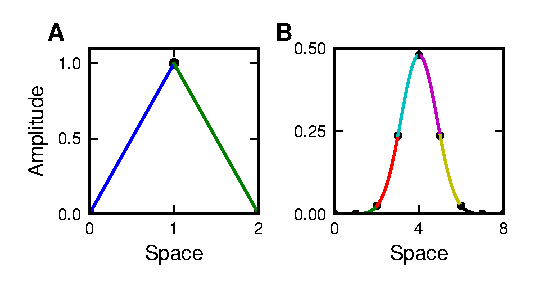
\includegraphics{./Graph/Figure0.pdf}
% 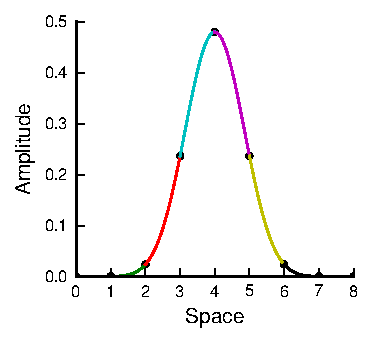
\includegraphics{./Graph/Figure0b.pdf}
\caption{{\bf Examples of cardinal B-spline functions}. Piecewise polynomial functions (coloured lines) are joined at the break points (black dots). (\textbf{A}) B-spline function of order 2 (linear B-spline). (\textbf{B}) B-spline function of order 8.}
\label{fig:Figure0}
\end{figure}
 
B-spline wavelet and scaling functions were formulated independently by \citet{Chui1992b,Chui1992,Unser1993}.  The scaling functions are $m$-th order B-splines and the compact support wavelet functions are a linear combination of scaling functions. B-spline wavelet and scaling functions approach optimal time/frequency localisation as the order of the spline increases. In fact, for the cubic B-spline scaling and wavelet functions it is already close to the optimal limit for Gaussian functions and they have a better approximation rate than other wavelets with the same number of vanishing moments \citep{Unser1999}. 

B-spline wavelet and scaling functions are particularly suited in this framework due to the property of being able to analytically define the convolution and inner product to form MRAIDE components. The following summarises some important characteristics of B-splines relevant to the proposed modelling framework. 

The $m$-th  order cardinal B-spline function is defined by the recurrence relation \citep{Chui1992} 
\begin{equation}
N_{m}\left(r\right) = \left(N_{m-1}\ast N_{1}\right)\left(r\right) = \int_0^{1} N_{m-1}\left( r-r'\right)\,\mathrm{d}r',
\label{SplineConvolutionIntegral}
\end{equation}
where $m>1$, $\ast$ denotes convolution, and $N_1\left(r\right)$ is the characteristic function of the unit interval $\left[ 0,1\right)$, also known as indicator function, i.e.
\begin{equation}
N_{1}\left(r\right)=
\begin{cases}
1 & \text{if $ 0\le r<1$}, \\
0 & \mathrm{elsewhere}.
\end{cases}
\end{equation}
Following this, a B-spline of any order, $N_m(r)$, can be computed using the recursive expression defined by \citep{DeBoor2001}
\begin{equation}\label{eq:MRA-DoBoorFormula}
 N_{m}\left(r\right)=\frac{r}{m-1}N_{m-1}\left(r\right)+\frac{m-r}{m-1}N_{m-1}\left(r-1\right) \quad m>1.
 \end{equation}
The most commonly used form of splines is the cubic spline $\left(m=4\right)$, comprised of third degree polynomials added together at the joining points, with an explicit expression given by
\begin{align}
3!N_{4}\left(r\right)=
\begin{cases}
r^3 & \text{if $ 0\le r\le1$}, \\
4-12r+12r^2-3r^3 & \text{if $1\le r\le2$}, \\
-44+60r-24r^2+3r^3 & \text{if $2\le r\le3$}, \\
64-48r+12r^2-r^3 & \text{if $3\le r\le4$}, \\
0 & \mathrm{elsewhere}.
\end{cases}
\end{align}
\parham{One important feature of the B-spline functions is the \emph{partition of unity} property, meaning that the unity can be expressed as a linear sum of B-splines, i.e
\begin{equation}
	\sum_{l}N_m(r+l)\equiv1
	\end{equation}
	This is important as the underlying field can be reconstructed in saturation without introducing numerical errors which is not the case for example in the case of Gaussian basis functions. }
	
The convolution and inner product of B-spline functions are required in order to formulate the multi-resolution framework described in the previous section (construction of $\boldsymbol\Lambda_{x}$, $\boldsymbol\Gamma$ and $\boldsymbol\Sigma_w$). To show how the convolution of two B-splines is calculated, \eqref{SplineConvolutionIntegral} can be rewritten as $(m-1)$ convolutions of the indicator function with itself
\begin{equation}\label{eq:N1convolutions}
 N_{m}\left(r\right)=\underbrace{\left(N_{1}\ast N_{1}\ast \cdots \ast N_{1}\right)}_{m-1\quad \text{convolutions}}\left(r\right).
\end{equation}
Using the associativity property of convolution, we have
\setlength{\arraycolsep}{0.0em}
\begin{align}\label{eq:BsplineConvolution}
N_{m}\left( r\right) \ast N_{m'}\left(r\right)&=\underbrace{\overbrace{\left(N_{1} \ast \cdots \ast N_{1}\right)}^{m-1 \quad \text{convolutions}}\left(r\right) \ast \overbrace{\left(N_{1} \ast \cdots \ast N_{1}\right)}^{m'-1\quad \text{convolutions}}}_{m+m'-1 \quad \text{convolutions}}\left(r\right)\nonumber\\
&=N_{m+m'}\left(r\right).
\end{align}
A direct consequence of \eqref{eq:BsplineConvolution} is the inner product between two B-splines is another translated B-spline such that
\begin{align}
 \left\langle N_{m}\left(r-l_{1}\right), N_{m'}\left(r-l_{2}\right)\right\rangle=&N_{m+m'}\left(m+l_{1}-l_{2}\right)\nonumber \\
=&N_{m+m'}\left(m'+l_{2}-l_{1}\right),
\label{eq:BsplineInnerProduct}
\end{align}
where $\left\langle \cdot,\cdot\right\rangle $ denotes the inner product. This holds as the support of $N_m\left(r\right)$ is $\left[ 0,m\right]$ and  is symmetric with respect to $r=\frac{m}{2}$, i.e. $ N_{m}\left(\frac{m}{2}+r\right)=N_{m}\left(\frac{m}{2}-r\right)$ (see Appendix~\ref{ap:InnerProductOfBsplines} for explicit derivation). The values of $N_{m+m'}$ in \eqref{eq:BsplineInnerProduct} can be easily determined recursively by evaluating \eqref{eq:MRA-DoBoorFormula} at integer points, i.e.
 \begin{equation}\label{eq:MRA-recursiveBsplineatintegerpoints}
 \begin{cases}
 N_2(k)=\delta(k-1)\quad k\in \mathbb{Z}, \\
 N_{m}\left(k\right)=\frac{k}{m-1}N_{m-1}\left(k\right)+\frac{m-k}{m-1}N_{m-1}\left(k-1\right) \quad k=1,2,\dots,m-1
  \end{cases}
 \end{equation}
Note $N_{m}\left(k\right)=0$ for $k\le0$ or $k\ge m$. 

The multi-resolution approximation using B-spline functions is completed by defining a two-scale relation pair, which relates the scaling functions and the wavelets at a given scale with the scaling function at the next higher scale. For cardinal B-spline scaling and wavelet functions of order $m$ the two-scale relation pair takes the form of
\begin{align}
 N_{m}\left(r\right)&=\sum_{n=0}^{m} \left[\mathbf p\right]_n N_{m}\left(2r-n\right) \label{eq:MRA-TwoScalepair1} \\
  \varphi_{m}\left(r\right) &= \sum_{n=0}^{3m-2} \frac{\left(-1\right)^n}{2^{m-1}} \left[\mathbf q\right]_n N_{m}\left(2r-n\right)\label{eq:MRA-TwoScalepair2},
 \end{align}
where 
 \begin{align}
\left[\mathbf p\right]_n&=2^{-m+1} \binom{m}{n} \quad \text{ $0\le n\le m$} \label{eq:MRA-TwoScalepair1coefs}\\
\left[\mathbf q\right]_n&= \sum_{l=0}^{m} \binom{m}{l} N_{2m}\left(n-l+1\right), \,  \text{ $0\le n\le 3m-2$}\label{eq:MRA-TwoScalepair2coefs}
 \end{align}
and $\left[\cdot\right]_n$ denotes the $n$-th element of the vector coefficients \citep{Chui1992}. \dean{Need to explicitly say why this is important and what this gives us here.}

Figure~\ref{fig:MRA-Figure1} shows the cubic B-spline scaling function and its associated wavelet function with dilation and translation parameters set to zero. Note in general the supports of the scaling and wavelet functions are given by 
\begin{align}
	\mathrm{supp}(N_{m;j,l})&=\left[\frac{l}{2^j},\frac{m+l}{2^j}\right] \\  
  \mathrm{supp}(\varphi_{m;j,l})&=\left[\frac{l}{2^j},\frac{2m-1+l}{2^j}\right] 
	\end{align} 
\begin{figure}[!t]
\centering
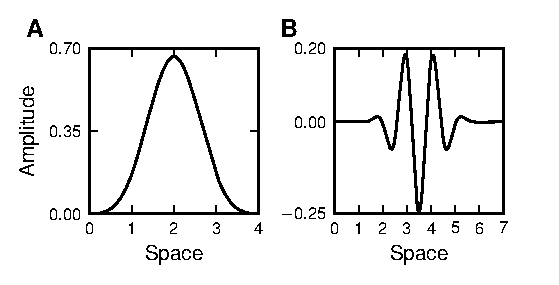
\includegraphics{./Graph/Figure1.pdf}
% 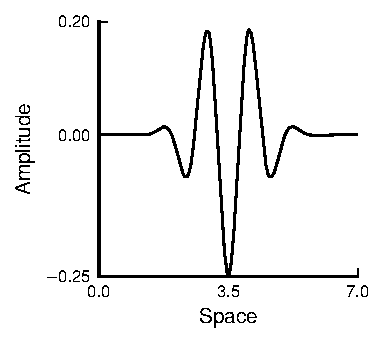
\includegraphics{./Graph/Figure1b.pdf}
\caption{{\bf Examples of B-spline scaling and wavelet functions}. (\textbf{A}) The cubic B-spline scaling function. (\textbf{B}) The corresponding wavelet function.}
\label{fig:MRA-Figure1}
\end{figure}

By exploiting \eqref{eq:BsplineConvolution} and \eqref{eq:BsplineInnerProduct}, the integrals in \eqref{eq:Lambdax}, \eqref{eq:Lambdatheta} and \eqref{eq:CovMatrix} can be computed analytically. In constructing $\boldsymbol\Lambda_{x}$, it is important to note that B-spline scaling and wavelet functions possess the following orthogonality properties \citep{Unser1993}: 
\begin{equation}
  \left\langle \varphi_{m;j_1,l_1}(r),\varphi_{m;j_2,l_2}(r)\right\rangle =0  \quad \mathrm{for} \quad j_1\neq j_2
 \label{eq:MRA-PsiPsiOrthogonality} 
 \end{equation}
 \begin{equation}
  \left\langle N_{m;j_1,l_1}(r),\varphi_{m;j_2,l_2}(r)\right\rangle =0  \quad \mathrm{for} \quad j_1\leq j_2.
 \label{eq:MRA-PhiPsiOrthogonality}
 \end{equation}
  \parham{Note from \eqref{eq:MRA-PsiPsiOrthogonality} Bspline wavelets are semiorthogonal as they are not orthogonal with respect to translation on a given scale.} 

In order to analytically calculate elements of $\boldsymbol\Lambda_{x}$ and $\boldsymbol\Lambda_{\theta}$, the scaling and wavelet basis functions must be expanded in terms of $N_m$ at the appropriate scale using the two-scale relation pair defined in equations (\ref{eq:MRA-TwoScalepair1}-\ref{eq:MRA-TwoScalepair2coefs}). For scaling functions this can be done  by using \eqref{eq:MRA-TwoScalepair1} recursively, giving
\begin{align}\label{eq:MRA-ConvertingFormulaForscalingFunctions}
 &N_m(r)=\nonumber \\
&\sum_{n_1,n_2, \dots n_j=0}^{m}\left[\mathbf p\right]_{n_1} \left[\mathbf p\right]_{n_2}\dots \left[\mathbf p\right]_{n_j}N_m(2^jr-l_{n_1,n_2, \dots, n_j}),
\end{align}
where 
\begin{align}
 l_{n_1,n_2, \dots, n_j}=2^{j-1}n_1+2^{j-2}n_2+ \dots +2^{0}n_j.
\end{align}
The relation \eqref{eq:MRA-ConvertingFormulaForscalingFunctions} can be also proven by induction (see Appendix ...). A similar method can be used for wavelet functions noting that they must be written first in terms of scaling functions using \eqref{eq:MRA-TwoScalepair2}. Examples of such expansions are given in Figure~\ref{fig:MRA-BasisDecomposition} where the scaling and wavelet functions at $j=0$ are written in terms of 625 and 1250 scaling functions at $j=4$ respectively.
\begin{figure}[!t] 
 	\centering
 		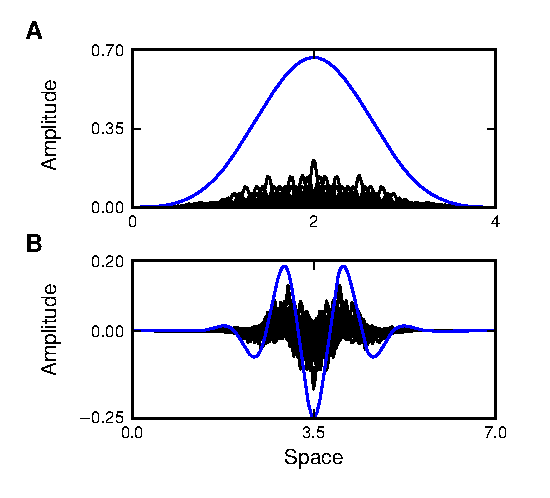
\includegraphics[scale=1]{./Graph/Decomposition.pdf}
 		\caption{{\bf The scaling and the wavelet function decomposition}. (\textbf{A}) The scaling function (blue) at $j=0$ is obtained using 625 scaling functions (black) at $j=4$. (\textbf{B}) The wavelet function (blue) at $j=0$ is obtained using 1250 scaling functions (black) at $j=4$.}
 	\label{fig:MRA-BasisDecomposition}
 \end{figure}  
 In this paper, 4th -- order cardinal B-spline scaling and wavelet functions are used, resulting in  8th and 12th order B-spline functions when calculating \eqref{eq:Lambdax}, \eqref{eq:Lambdatheta} and \eqref{eq:CovMatrix} whose values at integer points are given in Table~\ref{table:MRA-BsplineatIntegerPoints}.
\begin {table}[t]
\begin{center}
	\begin{tabular}{lcccc}
	\hline \hline
	& $k$ & $3!N_{4}\left(k\right)$ & $7!N_{8}\left(k\right)$ & $11!N_{12}\left(k\right)$\\ 
	\hline 
	& 1 & $1$ & $1$ & $1$\\
	& 2 & $4$ & $120$ & $2,036$\\
	& 3 & $\space$ & $1,191$ & $152,637$\\
	& 4 & $\space$ & $2,416$ & $2,203,488$\\
	& 5 & $\space$ & $\space$ & $9,738,114$\\
	& 6 & $\space$ & $\space$ & $15,724,248$\\
	\hline \hline
	\end{tabular}
 \caption {{\bf Cardinal B-Splines at the knot sequence}. Table entries are calculated using \eqref{eq:MRA-recursiveBsplineatintegerpoints} and can be also found in \citet{Goswami1999}.} 
 \label{table:MRA-BsplineatIntegerPoints}
 \end{center}
 \end {table}

\subsection{Frequency Analysis}
To determine the level of approximation in the model, detailed in the previous section, that is the number of basis functions required to reconstruct the field, $v_t(r)$, the frequency response of the B-spline function needs to be computed by applying the Fourier transform to \eqref{eq:N1convolutions}. To proceed the Fourier transform of $N_1(r)$ is first calculated, 
\begin{align}\label{eq:MRA-N1Fouriertransform}
\mathcal F(N_1(r))&=\int_{-\infty}^{+\infty}N_1(r)\mathrm{exp}(-2\pi i \nu r)dr \nonumber \\
&=\int_{0}^{1} \mathrm{exp}(-2\pi i \nu r)dr \nonumber \\
&=\frac{1-\mathrm{exp}(-2\pi i \nu)}{2\pi i\nu}.
\end{align}
The convolution theorem states that the Fourier transform of the convolution of functions is equal to the product of their Fourier transforms. Therefore, taking Fourier transform of \eqref{eq:N1convolutions} and substituting \eqref{eq:MRA-N1Fouriertransform} for $\mathcal F(N_1(r)) $ yields
\begin{align}\label{eq:MRA-NmFouriertransform}
\mathcal F(N_m(r))=\left(\frac{1-\mathrm{exp}(-2\pi i \nu)}{2\pi i\nu}\right)^m.
\end{align}
\dean{Need to say how the FT is used somewhere here before proceeding.} \parham{The Fourier transform of the $m$-th order Bspline allows the calculation of the spatial frequency response of the wavelets using \eqref{eq:MRA-TwoScalepair2} from which the level of approximation, $j$, can be determined. This way we choose wavelets upto level $j$ which fully describe the spatial frequency contents of the underlying neural field estimated from observations.}


\section{State and Parameter Estimation}
There exist many variations of state and parameter estimation methods for state-space models. The choice of algorithm is normally determined by the dimension of the system, whether the system is linear or nonlinear and whether or not the parameters are considered static or dynamic. Up to this point of the paper, we have not made any assumptions on any of these criteria for choosing an estimation algorithm. The MRAIDE neural field model formulation may be used in any of the above scenarios. 

To demonstrate the MRAIDE framework we shall consider the parameters to be static and we shall also assume that the relationship between the mean membrane potential and the mean firing rate is predominantly linear. Note that there is a difference between forward and inverse modelling when making these assumptions. For example, by using a linear activation function in the estimator we are not assuming that there is necessarily a linear relationship between the membrane voltage and firing rate, but that the statistics of the neural masses fall within a linear operating region over the estimation time period. 

It is important to point out there is no doubt that there will always be a mismatch between neural mass models and actual cortical tissue. Nevertheless, the simplifications used in formulating the equation enable the development of new methods for extracting information from electrophysiological data, that has the potential to influence the treatment of diseases such as epilepsy. The trade-off between parsimony and complexity is always difficult when considering neurodynamics and this is further complicated when using estimation algorithms that have huge computational demands with such high-dimensional systems.

By assuming a linear activation function of the form
\begin{equation}
	f(v_t(\mathbf{r})) = \varsigma v_t(\mathbf{r})
\end{equation}
the state transition equation~\eqref{eq:ApproxDiscreteTimeModel4} simplifies to
\begin{equation}\label{eq:ApproxDiscreteTimeModel_Linear}
	\mathbf{x}_{t+1} = 
	\xi \mathbf{x}_t + 
	\varsigma T_s \mathbf{\Lambda}_{x}^{-1} \int_{\Omega}\boldsymbol\mu\left(\mathbf{r}\right)\int_\Omega { 
	    \boldsymbol\theta^\top\boldsymbol\lambda\left(\mathbf{r}-\mathbf{r}'\right)
	    \boldsymbol\mu^\top\left(\mathbf{r}'\right) 
	\, \mathrm{d}\mathbf{r}'\mathrm{d}\mathbf{r}} \mathbf{x}_t
	+ \mathbf{w}_t.
\end{equation}
Now we can further simplify the system by defining
\begin{align}
	\label{eq:Lambdatheta}
	 \mathbf{\Lambda}_{\theta} &\triangleq \int_{\Omega}\boldsymbol\mu\left(r\right) \int_\Omega { 
		   \boldsymbol\theta^\top\boldsymbol\lambda\left(r-r'\right)
		    \boldsymbol\mu^\top\left(r\right)\ \mathrm{d}r'\mathrm{d}r}
\end{align}
to give the state transition equation
\begin{align}\label{eq:StateEquation}
 \mathbf x_{t+1} &=\mathbf A(\boldsymbol \theta) \mathbf x_t+ \mathbf w_t\\
\label{eq:A_theta}
 \mathbf A(\boldsymbol \theta) &= T_s\varsigma\mathbf{\Lambda}_{x}^{-1}\mathbf{\Lambda}_{\theta}+\xi\mathbf I.
\end{align} 
The problem of joint state and parameter estimation for the state-space model given by \eqref{eq:StateEquation} and \eqref{eq:ReducedObservationEquation} can be formulated as 
\begin{equation}
	{\hat{\mathbf X},\hat{\boldsymbol\theta}}=\arg\max_{\mathbf X,\boldsymbol\theta}p(\mathbf Y;\boldsymbol\theta),
 \end{equation}  
where $\mathbf X$ and $\mathbf Y$ denote the entire sequences of the states and observations respectively, $\boldsymbol\theta$ is the parameter set and $p(\mathbf Y;\boldsymbol\theta)$ denotes the probability density function of the observations parameterised  by $\boldsymbol\theta$, known as the likelihood function. This problem cannot be solved separately as for the state estimation the knowledge of the system's parameters is required and for the parameter estimation the states of the system need to be known. One approach is to iteratively estimate the states and parameters of the system and monitor the convergence of the algorithm. A natural framework to perform this is the well known Expectation Maximisation (EM) algorithm \cite{Dempster1977,Shumway2000} to infer both the parameter set and the states from the observations corresponding to the connectivity kernel, the neural field and electrophysiological data in our application. There are two main applications of the EM algorithm:  first is when the observations are incomplete due to a faulty observation process or existing limitations and the second  when the direct maximisation of the likelihood function is difficult but can be simplified by assuming the existence of an additional however missing (or hidden) variables \cite{Bilmes1998}, the weights of the field basis functions in this case. The EM algorithm, when used in the latter context \cite{Dewar2009}, yields the maximum likelihood kernel estimate, i.e.
\begin{equation}
	\boldsymbol\theta_{\text{ML}}=\arg\max_{\boldsymbol\theta}~p(\mathbf Y;\boldsymbol\theta),
 \end{equation}   
and the posterior distribution of the field over time.

Both the E and the M steps of the EM algorithm find increasingly tighter lower bounds on the likelihood of the parameters so that, at convergence, the maximum of the bound corresponds to the maximum of the likelihood. For state-space models, the E-step corresponds to the smoothing problem which can be solved using the Rauch Tung Streibel (RTS) smoother \cite{RAUCH1965}. For the M-step, a lower bound on the likelihood function should be constructed where the steps needed
to compute the required quantities are very dependent on the particular application which is described in detail for our problem. 

In summary, to solve the joint state and parameter estimation for linear state-space models one can adapt the EM algorithm, solving the smoothing problem for the E-step and constructing and maximising the lower bound in the M-step. A schematic representation of the EM algorithm is represented in Figure~\ref{fig:EMBlockDiagram}.  
\begin{figure}[!t]
\centering
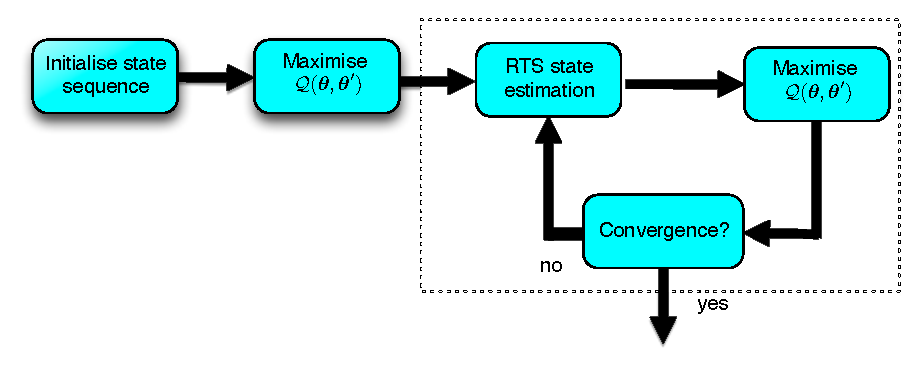
\includegraphics[scale=1]{./Graph/EMBlockDiagram.pdf}
\caption{{\bf Schematic of the EM algorithm}. The RTS smoother (E-step) and the maximisation of the lower bound, $\mathcal Q(\boldsymbol \theta,\boldsymbol\theta')$, (M-step) are shown. The dashed box shows the iterative two step algorithm once it is initialised.}
\label{fig:EMBlockDiagram}
\end{figure}
  \subsection{E-step}
  As mentioned earlier the E-step for state-space models is equivalent to the smoothing problem. We use the RTS smoother in order to infer the states of the system. The RTS smoother uses the Kalman filter \cite{Kalman1960} in forward pass along withe a backward iteration to calculate its outputs: smoothed states $\hat{\mathbf x}^b_t$ and covariances, $\mathbf P^b_t=\mathrm{cov}(\mathbf{x}_t)$. Following \cite{Gibsona2005}, an additional backwards recursion is also included (step 6 of the RTS algorithm)	to calculate cross-covariance matrix, $\mathbf M_t=\mathrm{cov}(\mathbf{x}_{t},\mathbf{x}_{t+1})$, which is also required in forming the lower bound to be maximised in the M-step. Note that the following quantities from the forward iteration (filtering) should be stored when implementing the RTS smoother: predicted and corrected estimates for both state estimates ($\mathbf{x}_t^{f-}$, $\mathbf{x}_t^{f}$) and covariance matrices ($\mathbf P_t^{f-}$,$\mathbf P_t^f$). Also the final value of the Kalman gain, $\mathcal K_T$, should be stored in order to initialise the backward cross-covariance computation. 
 \subsection{M-step}
It is rather straightforward to show that 
\begin{equation}
	\mathcal Q(\boldsymbol \theta,\boldsymbol\theta')= \mathbf E_{\boldsymbol \theta'}\left[2\ln p(\mathbf X,\mathbf Y;\boldsymbol \theta)\right], 
\end{equation}
is a lower bound on the log-likelihood function \cite{Bishop2006} (see Appendix~\ref{ap:Lowerbound} )  where $p(\mathbf X,\mathbf Y;\boldsymbol \theta)$ is the joint probability distribution of the states and the observations and where $ \mathbf E_{\boldsymbol \theta'}\left[\cdot\right] $ denotes expectation taken with respect to the marginal distribution of the states conditioned on the observed field and the current estimate of the parameter set, $\boldsymbol\theta'$ i.e.  $p(\mathbf X\mid\mathbf Y;\boldsymbol \theta'$). Note that this is actually the smoother output.

 The rest of this section is to construct the lower bound $\mathcal Q$ for the linear state-space model given by \eqref{eq:StateEquation} and \eqref{eq:ReducedObservationEquation}. The joint probability distribution $p(\mathbf X,\mathbf Y;\boldsymbol \theta)$ can be written as
 \begin{equation}\label{eq:jointdistribution}
  p(\mathbf X,\mathbf Y;\boldsymbol \theta)=\prod_{t=0}^{T-1} p(\mathbf y_{t+1}|\mathbf x_{t+1})p(\mathbf x_{t+1}|\mathbf x_{t};\boldsymbol \theta)p(\mathbf x_0).
 \end{equation}
The $\mathcal Q$-function, or lower-bound on the likelihood, can be expressed in terms of the joint distribution components
 \begin{align}
  \mathcal Q(\boldsymbol \theta,\boldsymbol\theta')&=\mathbf E_{\boldsymbol \theta'}\left[2\ln p(\mathbf X,\mathbf Y;\boldsymbol \theta)\right] \nonumber \\
 &=\mathbf E_{\boldsymbol\theta'}\left[\sum_{t=0}^{T-1}2\ln p(\mathbf y_{t+1}|\mathbf x_{t+1})+\sum_{t=0}^{T-1}2\ln p(\mathbf x_{t+1}|\mathbf x_{t};\boldsymbol \theta)
 +\sum_{t=0}^{T-1}2\ln p(\mathbf x_0)\right],
 \end{align}   
It should be noted that neither $p(\mathbf y_{t+1}|\mathbf x_{t+1})$ nor $p(\mathbf x_0)$ are functions of the parameter set and therefore the $\mathcal Q$-function can be rewritten as
\begin{equation}
\mathcal Q(\boldsymbol \theta,\boldsymbol\theta')=\mathbf E_{\Theta'}\left[\sum_{t=0}^{T-1}2\ln p(\mathbf x_{t+1}|\mathbf x_{t};\boldsymbol \theta)\right]+\mathrm{const.}
\end{equation}
where the constant term can be ignored as it is independent of the parameters. Under the condition that the state distribution is Gaussian --- ignoring the normalising term, $1/(2\pi)^{\frac{n_x}{2}}\mid\boldsymbol\Sigma_w\mid^{-\frac{1}{2}}$ --- the conditional distribution $p(\mathbf x_{t+1} | \mathbf x_{t};\boldsymbol\theta)$ can be written as
\begin{align}
p(\mathbf x_{t+1} | \mathbf x_{t};\boldsymbol\theta)=  \exp\left({-\frac{1}{2}\left(\mathbf x_{t+1}-\mathbf A\left(\boldsymbol\theta\right)\mathbf  x_t\right)^\top\boldsymbol\Sigma_w^{-1}\left(\mathbf x_{t+1}-\mathbf A\left(\boldsymbol\theta\right)\mathbf  x_t\right)}\right).
\end{align}
Twice the logarithm of the above distribution, once expanded, is given by
\begin{align}\label{eq:Qfunction}
2\ln p(\mathbf x_{t+1} , \mathbf y_{t+1};\boldsymbol\theta)=&-\mathbf x_{t+1}^\top\boldsymbol\Sigma_w^{-1}\mathbf x_{t+1}+2\mathbf x_{t+1}^\top\boldsymbol\Sigma_w^{-1}\mathbf A( \boldsymbol\theta)\mathbf x_t\nonumber \\
&-\mathbf x_t^\top\mathbf A^\top(\boldsymbol\theta)\boldsymbol\Sigma_w^{-1}\mathbf A(\boldsymbol\theta)\mathbf x_t.
\end{align}
Substituting $\mathbf A( \boldsymbol\theta)$ from \eqref{eq:A_theta} into \eqref{eq:Qfunction} gives
\begin{align}
2\ln p(\mathbf x_{t+1}, \mathbf y_{t+1};\boldsymbol\theta)=&\beta+2 T_s\varsigma\mathbf x_{t+1}^\top\boldsymbol\Sigma_w^{-1}\boldsymbol\Lambda_x^{-1}\boldsymbol\Lambda_{\theta}\mathbf x_t \nonumber \\
&-T_s^2\varsigma^2\mathbf x_t^\top \boldsymbol\Lambda_{\theta}^\top\boldsymbol\Lambda_x^{-1}\boldsymbol\Sigma_w^{-1}\boldsymbol\Lambda_x^{-1}\boldsymbol\Lambda_{\theta}\mathbf x_t-2\xi \varsigma T_s\mathbf x_t^\top\boldsymbol\Sigma_w^{-1}\boldsymbol\Lambda_x^{-1}\boldsymbol\Lambda_{\theta}\mathbf x_t,\nonumber \\
\end{align}
where 
\begin{equation}
\beta=-\mathbf x_{t+1}^\top\boldsymbol\Sigma_w^{-1}\mathbf x_{t+1}+2\xi\mathbf x_{t+1}^\top\boldsymbol\Sigma_w^{-1}\mathbf x_t-\xi^2\mathbf x_t^\top\boldsymbol\Sigma_w^{-1}\mathbf x_t,
\end{equation}
is constant with respect to parameter $\boldsymbol\theta$ and will disappear subject to differentiation with respect to $\boldsymbol\theta$. Taking the trace and rearranging, using the invariant cyclic permutations property of the trace, this distribution can be written as
\begin{align}\label{eq:Qfunctionintrace}
2\ln p(\mathbf x_{t+1}, \mathbf y_{t+1};\boldsymbol\theta)&=\beta+2 T_s\varsigma\mathrm{tr} \left\lbrace \mathbf x_t\mathbf x_{t+1}^\top\boldsymbol\Sigma_w^{-1}\boldsymbol\Lambda_x^{-1}\boldsymbol\Lambda_{\theta}\right\rbrace \nonumber \\
&-T_s^2\varsigma^2\mathrm{tr} \left\lbrace \mathbf x_t\mathbf x_t^\top \boldsymbol\Lambda_{\theta}^\top\boldsymbol\Lambda_x^{-1}\boldsymbol\Sigma_w^{-1}\boldsymbol\Lambda_x^{-1}\boldsymbol\Lambda_{\theta}\right\rbrace\nonumber \\
&-2\xi\varsigma T_s\mathrm{tr} \left\lbrace \mathbf x_t\mathbf x_{t}^\top\boldsymbol\Sigma_w^{-1}\boldsymbol\Lambda_x^{-1}\boldsymbol\Lambda_{\theta}\right\rbrace.
\end{align}
Rearranging and taking the expectation of the log-likelihood function over all time instants gives the required lower-bound which is to be maximised for the optimal parameter estimates. Note that the expectation distributes over the trace sum. Therefore, 
\begin{align}\label{eq:MRA-QintermsofTraces}
\mathcal Q(\boldsymbol \theta, \boldsymbol\theta')&=\beta+2 T_s\varsigma\mathrm{tr} \left\lbrace \boldsymbol \Xi_0\boldsymbol\Sigma_w^{-1}\boldsymbol\Lambda_x^{-1}\boldsymbol\Lambda_{\theta}\right\rbrace-2\xi\varsigma T_s\mathrm{tr} \left\lbrace \boldsymbol\Xi_1\boldsymbol\Sigma_w^{-1}\boldsymbol\Lambda_x^{-1}\boldsymbol\Lambda_{\theta}\right\rbrace \nonumber \\
&-T_s^2\varsigma^2\mathrm{tr} \left\lbrace \boldsymbol\Xi_1 \boldsymbol\Lambda_{\theta}^\top\boldsymbol\Lambda_x^{-1}\boldsymbol\Sigma_w^{-1}\boldsymbol\Lambda_x^{-1}\boldsymbol\Lambda_{\theta}\right\rbrace,
\end{align}
where
\begin{align}
\boldsymbol\Xi_0&=\mathbf E_{\Theta'}\left[\sum_{t=0}^{T-1}\mathbf x_t\mathbf x_{t+1}^\top\right] \label{eq:MRA-Xi0}\\
\boldsymbol\Xi_1&=\mathbf E_{\Theta'}\left[\sum_{t=0}^{T-1}\mathbf x_t\mathbf x_{t}^\top\right] \label{eq:MRA-Xi1}.
\end{align}
The matrices $\boldsymbol\Xi_0$ and $\boldsymbol\Xi_1$ are calculated using the RTS smoother outputs: $\hat{\mathbf x}_t$, covariance, $\mathbf P_t^b$, and cross-covariance matrix, $\mathbf M_t$ \cite{Gibsona2005}, (see Appendix~\ref{ap:Xiderivation} for more details)
\begin{align}
\boldsymbol\Xi_0&=\sum_{t=0}^{T-1}\left(\mathbf M_{t+1}+\mathbf{\hat x}_t\mathbf{\hat x}_{t+1}^\top\right) \label{eq:Xi0} \\
 \boldsymbol\Xi_1&=\sum_{t=0}^{T-1}\left(\mathbf P_t+\mathbf{\hat x}_t\mathbf{\hat x}_t^\top\right).  \label{eq:Xi1}
\end{align} 

The three traces that form \eqref{eq:MRA-QintermsofTraces} are dealt with in turn. To begin, the first trace is written in terms of element-wise summations
\begin{align}\label{eq:MRA-trace1}
\mathrm{tr} \left\lbrace \boldsymbol \Xi_0\boldsymbol\Sigma_w^{-1}\boldsymbol\Lambda_x^{-1}\boldsymbol\Lambda_{\theta}\right\rbrace&=\sum_{i=1}^{n_x}\left[ \boldsymbol \Xi_0\boldsymbol\Sigma_w^{-1}\boldsymbol\Lambda_x^{-1}\boldsymbol\Lambda_{\theta}\right]_{ii} \nonumber \\
&=\sum_{i,j=1}^{n_x}\left[ \boldsymbol\Xi_0\right]_{ij}\left[\boldsymbol\Sigma_w^{-1}\boldsymbol\Lambda_x^{-1}  \boldsymbol\Lambda_{\theta}\right]_{ji}\nonumber\\
&=\sum_{i,j=1}^{n_x}\left[ \boldsymbol\Xi_0\right]_{ij}\sum_{k=1}^{n_x}\left[\boldsymbol\Sigma_w^{-1}\boldsymbol\Lambda_x^{-1} \right]_{jk} \left[ \boldsymbol\Lambda_{\theta}\right]_{ki},
\end{align}
where $[\cdot]_{p,q}$ denotes the $\left(p,q\right)$-element of the matrix. Each element of $\boldsymbol\Lambda_{\theta}$ can be calculated using
\begin{equation}\label{eq:MRA-LambdaThetaElements}
\left[ \boldsymbol\Lambda_{\theta}\right] _{k,i}=\left[ \mathbf U\right]^{k,i}\boldsymbol\theta,
\end{equation}
where $ [\cdot]^{p,q}$ denotes the $\left(p,q\right)$-block of the block matrix, and where
each $ 1 \times n_{\theta}$ block of the $n_x \times n_x n_{\theta}$ block matrix $\mathbf U$ is 
\begin{align}
\left[ \mathbf U\right] ^{k,i}&=\int_{\boldsymbol \Omega}\left[\boldsymbol\mu(r) \right]_k \left[\int_{\boldsymbol\Omega} \boldsymbol\mu\left(r'\right)\boldsymbol \lambda^\top \left(r-r'\right) dr'\right]_{i:} dr,
\end{align}
where $[\cdot]_{i:} $ denotes the i-th row.  By substituting for $\left[ \boldsymbol\Lambda_{\theta}\right] _{k,i}$ from \eqref{eq:MRA-LambdaThetaElements} the trace given in \eqref{eq:MRA-trace1} can be written as
\begin{align}
\mathrm{tr} \left\lbrace \boldsymbol \Xi_0\boldsymbol\Sigma_w^{-1}\boldsymbol\Lambda_x^{-1}\boldsymbol\Lambda_{\theta}\right\rbrace&=\sum_{i,j=1}^{n_x}\left[ \boldsymbol\Xi_0\right]_{ij}\sum_{k=1}^{n_x}\left[ \boldsymbol\Sigma_w^{-1}\boldsymbol\Lambda_x^{-1}\right]_{jk} \left[ \mathbf U\right]^{k,i}\boldsymbol\theta \nonumber \\
&=\sum_{i,j=1}^{n_x}\left[ \boldsymbol\Xi_0\right]_{ij}\left[ \Gamma_1\right] ^{j,i}\boldsymbol\theta
\end{align}
where
\begin{align}
\left[ \Gamma_1\right]^{j,i} =\sum_{k=1}^{n_x}\left[ \boldsymbol\Sigma_w^{-1}\boldsymbol\Lambda_x^{-1}\right]_{jk} \left[ \mathbf U\right]^{k,i}.
\end{align}
The second trace of \eqref{eq:MRA-QintermsofTraces} is dealt with in a similar manner, giving
\begin{align}
\mathrm{tr} \left\lbrace \boldsymbol \Xi_1\boldsymbol\Sigma_w^{-1}\boldsymbol\Lambda_x^{-1}\boldsymbol\Lambda_{\theta}\right\rbrace&=
\sum_{i,j=1}^{n_x}\left[ \boldsymbol\Xi_1\right]_{ij}\left[ \Gamma_1\right] ^{j,i}\boldsymbol\theta.
\end{align}
Likewise, the third trace of \eqref{eq:MRA-QintermsofTraces} is broken down into element-wise summations
\begin{align}
\mathrm{tr} \left\lbrace \boldsymbol\Xi_1 \boldsymbol\Lambda_{\theta}^\top\boldsymbol\Lambda_x^{-1}\boldsymbol\Sigma_w^{-1}\boldsymbol\Lambda_x^{-1}\boldsymbol\Lambda_{\theta}\right\rbrace&=\sum_{i,j,k,m=1}^{n_x}\left[\boldsymbol\Xi_1\right] _{i,j}[\boldsymbol\Lambda_{\theta}^{\top}]_{jk} \left[\boldsymbol\Lambda_x^{-1}\boldsymbol\Sigma_w^{-1}\boldsymbol\Lambda_x^{-1} \right]_{km}[\boldsymbol\Lambda_{\theta}]_{mi} \nonumber \\
=&\boldsymbol\theta^\top\sum_{i,j=1}^{n_x}\left[\boldsymbol\Xi_1\right] _{i,j}\sum_{k,m=1}^{n_x}[\mathbf U^{\top}]^{jk} \left[\boldsymbol\Lambda_x^{-1}\boldsymbol\Sigma_w^{-1}\boldsymbol\Lambda_x^{-1} \right]_{km}[\mathbf U]^{mi}~\boldsymbol\theta \nonumber \\
&=\boldsymbol\theta^\top\sum_{i,j=1}^{n_x}\left[\boldsymbol\Xi_1\right] _{i,j}\left[ \Gamma_2\right] ^{j,i}\boldsymbol\theta,
\end{align}
where
\begin{align}
\left[ \Gamma_2\right] ^{j,i}=\sum_{k,m=1}^{n_x}[\mathbf U^{\top}]^{jk} \left[\boldsymbol\Lambda_x^{-1}\boldsymbol\Sigma_w^{-1}\boldsymbol\Lambda_x^{-1} \right]_{km}[\mathbf U]^{mi}.
\end{align}
Therefore the $\mathcal Q$-function can be rewritten as
\begin{equation}\label{eq:MRA-QCompact}
\mathcal Q\left(\boldsymbol \theta,\boldsymbol\theta'\right)=\beta+2T_s\varsigma\left(\boldsymbol\upsilon_0-\boldsymbol\upsilon_1\right)\boldsymbol\theta-T_s\varsigma\boldsymbol\theta^\top\boldsymbol\Upsilon\boldsymbol\theta,
\end{equation}
where
\begin{equation}\label{eq:epsilon0}
\boldsymbol\upsilon_0=\sum_{i,j=1}^{n_x}[\boldsymbol\Xi_0]_{i,j}[\boldsymbol\Gamma_1]_{j,i}
\end{equation}
and
\begin{equation}\label{eq:epsilon1}
\boldsymbol\upsilon_1=\xi\sum_{i,j=1}^{n_x}[\boldsymbol\Xi_1]_{i,j}[\boldsymbol\Gamma_1]^{j,i}
\end{equation}
\begin{equation}\label{eq:Epsilon}
\boldsymbol\Upsilon=T_s\varsigma\sum_{i,j=1}^{n_x}[\boldsymbol\Xi_1]_{i,j}[\boldsymbol\Gamma_2]^{j,i}
\end{equation}
All $n_x^2$ blocks of $\boldsymbol\Gamma_1$ and $\boldsymbol\Gamma_2$  can be computed as a one-off before the commencement of the EM iterations, which increases the speed of the M-step significantly compared to the implementation in \citet{Dewar2009}. The complexity of each step of the algorithm is summarised in Table~\ref{table:MRA-ComputationalComplexity} where for ease of comparison the computational complexity of the method in \citet{Dewar2009} is also identified.
\begin {table}
\begin{center}
\scalebox{1}{\begin{tabular}{lllc}
\hline \hline
Variable &Equation&Order&Order obtained from \citet{Dewar2009}\\ \hline\\
$\Xi_0, \Xi_1$&\eqref{eq:MRA-Xi0}, \eqref{eq:MRA-Xi1}&$O(Tn_x^2)$& -\\
$\boldsymbol\upsilon_0, \boldsymbol\upsilon_1$&\eqref{eq:epsilon0},\eqref{eq:epsilon1} &$O(n_x^2n_{\theta})$ &$O(n_x^2n_{\theta})+O(n_x^3)$ \\
$\boldsymbol\Upsilon$&\eqref{eq:Epsilon}&$O(n_x^2n_{\theta}^2)$&$O(n_x^4n_{\theta}^2)$\\
$\mathbf A(\boldsymbol\theta)$&\eqref{eq:A_theta}&$O(n_x^3)$&-\\
$\boldsymbol\Lambda_{\theta}$&\eqref{eq:Lambdatheta}&$O(n_x^2n_{\theta})$&-\\
$\hat{\boldsymbol\theta} $&\eqref{eq:MRA-thetahat}&$O(n_{\theta}^3)$&-\\
\hline \hline
\end{tabular}}
 \caption {{\bf The Computational complexity of the estimation algorithm}. A comparison between the algorithm proposed herein and that of \citet{Dewar2009}.} 
\label{table:MRA-ComputationalComplexity}
\end{center}
\end {table}

By differentiating the $\mathcal Q$-function with respect to $\boldsymbol\theta$ we have
\begin{align}\label{eq:MRA-QDerivative}
\frac{\partial \mathcal Q}{\partial \boldsymbol\theta}&=2T_s\varsigma(\boldsymbol\upsilon_0-\boldsymbol\upsilon_1)^\top-T_s\varsigma(\boldsymbol\Upsilon^\top+\boldsymbol\Upsilon)\boldsymbol\theta \nonumber \\
&=2T_s\varsigma(\boldsymbol\upsilon_0-\boldsymbol\upsilon_1)^\top-2T_s\varsigma\boldsymbol\Upsilon^\top\boldsymbol\theta.
\end{align}
Equating \eqref{eq:MRA-QDerivative} to $\mathbf 0$ yields
\begin{align}\label{eq:MRA-thetahat}
\boldsymbol \theta= \boldsymbol\Upsilon^{-\top}(\boldsymbol\upsilon_0-\boldsymbol\upsilon_1)^\top.
\end{align}
The second derivative of the $\mathcal Q$-function is given by
\begin{equation}
\frac{\partial^2\mathcal Q}{\partial\boldsymbol\theta^2}=-2T_s\varsigma\boldsymbol\Upsilon.
\end{equation}
The matrix $\boldsymbol\Upsilon$ is positive definite if $n_x^2\times n_{\theta}$ matrix $\mathrm{vec}(\mathbf U)$ is of rank $n_{\theta}$ (\citep{Dewar2009}, Lemma 3), where $\mathrm{vec}(\cdot)$ denotes the vectorization operator. Under this condition $\boldsymbol\Upsilon$ is  invertible and the second derivative is negative definite representing a maximum of the $\mathcal Q$-function. 


The algorithm has two steps: the E-step, which computes $\boldsymbol\Xi_0$ and $\boldsymbol\Xi_1$ based on the most recent parameter estimates using the RTS smoother, and the M-step, which updates the parameter estimates by computing the (analytic) maximum of $Q(\boldsymbol\theta,\boldsymbol\theta')$. The EM algorithm iterates between these two steps until the parameter estimates converge. The RTS  algorithm is given in Algorithm~\ref{alg:MRA-RTS} for completeness. 
\begin{algorithm}
\caption{Summary of the Rauch-Tung-Striebel smoother}
\label{alg:MRA-RTS}
 % \begin{tabbing}
 \begin{enumerate}
 \item Forward initialisation: 
 \begin{equation*}
 \hat{\mathbf x}_0, \mathbf P_0
 \end{equation*}
 \item Forward iteration: for $t\in\left\lbrace 0,\cdots,T\right\rbrace $, calculate the predicted state and the predicted covariance matrix
 \begin{align}
 \hat{\mathbf x}_{t+1}^{f-}&=\mathbf A \hat{\mathbf x}_{t}^{f} \nonumber \\
 \mathbf P_{t+1}^{f-}&=\mathbf A \mathbf P_{t}^{f}\mathbf A^{\top}+\boldsymbol\Sigma_e \nonumber 
 \end{align}
 \item Compute the filter gain, the filtered state and the filtered covariance matrix
 \begin{align}
 \mathcal K_{t+1}&=\mathbf P_{t +1}^{f-}\mathbf C ^\top(\mathbf C \mathbf P_{t +1}^{f-}\mathbf C ^\top+\boldsymbol \Sigma_{\varepsilon})^{-1} \nonumber\\
\hat{\mathbf x}_{t+1}^{f}&=\hat{\mathbf x}_{t+1}^{f-}+\mathcal K_{t+1}(\mathbf y_{t+1}-\mathbf C\hat{\mathbf x}_{t +1}^{f-})\nonumber \\
 \mathbf P_{t+1}^f&=(\mathbf I - \mathcal K_{t+1}\mathbf C)\mathbf P_{t +1}^{f-} \nonumber 
 \end{align}
 \item  Backward initialisation:
 \begin{equation*}
 \mathbf P_T^b= \mathbf P_T^f, \quad \hat{\mathbf x}^b_T= \hat{\mathbf x}^f_T
 \end{equation*}
 \item Backward iteration: for $t\in\left\lbrace T-1,\cdots,0\right\rbrace $ compute the smoother gain, the smoothed state and the smoothed covariance matrix
 \begin{align}
  \mathbf S_{t}&=\mathbf P_{t}^{f}\mathbf A^{\top}\left[ \mathbf P_{t +1}^{f-}\right]^{-1} \nonumber\\
 \hat{\mathbf x}_t^b&=\hat{\mathbf x}_t^f+\mathbf S_t(\hat{\mathbf x}_{t+1}^{b}-\hat{\mathbf x}_{t+1}^{f-})\nonumber \\
 \mathbf P_{t}^{b}&=\mathbf P_{t}^{f}+\mathbf S_t(\mathbf P_{t+1}^{b}-\mathbf P_{t+1}^{f-})\mathbf S_t^\top \nonumber
 \end{align}
 \item compute the smoothed cross covariance matrix\\
 initialisation:
 \begin{align}
  \mathbf M_T=(\mathbf I-\mathcal K_T\mathbf C)\mathbf A\mathbf P_{T-1}^b \nonumber
 \end{align}
 Backward iteration: for $t\in\left\lbrace T-1,\cdots,0\right\rbrace $
 \begin{align}
 \mathbf M_t= \mathbf P_t^{f}\mathbf S_{t-1}^{\top}+\mathbf S_{t}(\mathbf M_{t+1}-\mathbf A\mathbf P_t^{f} )\mathbf S_{t-1}^{\top}\nonumber
 \end{align}
 \end{enumerate}
 % \end{tabbing}
 \end{algorithm}
\subsection{Stopping rule}
The stopping criterion is usually associated with either the change in the parameter estimates or the log-likelihood variation \cite{McLachlan1997}. The stopping rule adopted herein is
\begin{equation}
 \left(\parallel \mathbf{A} \parallel_{F}^{(i)}-\parallel \mathbf{A} \parallel_{F}^{(i-1)}\right)<\epsilon,
 \end{equation}
 where $\epsilon$ is a threshold value and $\parallel \mathbf{A} \parallel_{F}^{(i)}$ and $ \parallel \mathbf{A} \parallel_{F}^{(i-1)}$ are the Frobenius norms  of the successive estimates of $\mathbf{A} $ matrices which is defined by \citet{Meyer2000}
 \begin{equation}
  \parallel \mathbf{A} \parallel_{F}=\sqrt{\sum_{i,j=1}^{n_x}\mid a_{i,j} \mid^2}=\sqrt{\mathrm{tr} (\mathbf A^{\top}\mathbf A)}
 \end{equation}
%\cut{The second terms in  \eqref{eq:upsilon0}, \eqref{eq:upsilon1}, and \eqref{eq:Upsilon} can be computed as a once-off before the commencement of the EM iterations, which increases the speed of the M-step significantly compared to the method in \cite{Dewar2009}.}

\section{Results}\label{sec:MRA-results}
To demonstrate the performance of the MRAIDE estimation framework, data was generated synthetically  using equations \eqref{eq:DiscreteTimeModel} and \eqref{eq:ObservationEquation}, allowing a comparison between true and estimated parameters. In doing so, the membrane time constant was set to $\tau = 10$~ms \citep{David2003}, and the sampling time was chosen ten times faster \citep{Stephan2008}, i.e. $T_s = 1$~ms, ensuring the discrepancy between the continuous neural field model and its discrete approximation is small. 

Two different experiments were designed to test the framework. In the first one, 200 realisations of 1 second of data were used, where the field disturbance, $e_t$, and the observation noise, $\boldsymbol\varepsilon_t$, were regenerated each run. This way the net shape of the connectivity kernel could be formed by averaging over the parameters estimates from each realisation. In the second experiment, a single data set was generated and the field estimations are compared for five models, each accounting for a different level of approximation, i.e. $j=0$ to $j=4$. 

For each of the experiments, the estimation was applied to the final 900~ms, allowing the forward model's dynamics to stabilise from the initial conditions. The initial state, parameters and the support of the connectivity kernel were unknown to the estimator. The observation noise was set to $\boldsymbol\Sigma_{\varepsilon}=0.1 \times \mathbf{I}_{n_y}$ and the disturbance covariance function was set to $\gamma(r-r') = \varphi_{3,-2}(r-r')$ (B-spline, $j=3$).  The firing rate slope, $\varsigma$ was set to $0.56~mV^{-1}$ \citep{Wendling2005}. The observation kernel was modelled using a B-spline function, with a width of 0.8~mm at half the maximum amplitude where the distance between adjacent sensors was $0.5$~mm, resulting into $n_y = 161$ observations. The spacing and bandwidth of the sensors allowed the full spatial bandwidth of the field to be observed.  With this number of observations, the estimation problem was well-posed, i.e. the number of states, $n_x < n_y$ at each level of the decomposition. This is because the scaling functions are orthogonal to the wavelets at the same and higher levels of decomposition, and  the wavelets are orthogonal to each other across different scales (see (\ref{eq:MRA-PsiPsiOrthogonality}-\ref{eq:MRA-PhiPsiOrthogonality})). 

\subsection{Experiment I}
The spatial frequency response of the observed field was used to specify the level of decomposition required to represent the field using the wavelets. This is shown in Figure~\ref{fig:ObservationFrequencyResponce} where the graph obtained by averaging the spectral power of the spatial frequency (over time) from the observations \citep{Scerri2009}. The spatial bandwidths of wavelets was calculated analytically using equation \eqref{eq:MRA-NmFouriertransform}. The result suggested that wavelets up to level $j=3$ (with the bandwidth $\approx[5,8]$ cycles/mm) can represent the significant spatial characteristics of the field which yields $n_x = 131$ states, corresponding to 9 scaling functions at $j=0$ and 8, 16, 32 and 66 wavelet functions, respectively at $j=0$, $j=1$, $j=2$ and $j=3$. 
\begin{figure}[!t] 
 	\centering
 		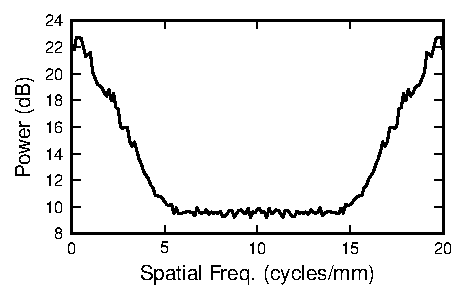
\includegraphics[scale=1]{./Graph/Figure2.pdf}
 		\caption{{\bf Spatial frequency analysis}. The average (over time) power in dB of the spatial frequency of the observations.}
 	\label{fig:ObservationFrequencyResponce}
 \end{figure}

The EM algorithm was allowed to run until a maximum number of 20 iterations was reached, though typically the change in the transition matrix Frobenius norm dropped below $10^{-6}$ after less than 10 iterations. The rate of convergence of the EM based algorithm is depicted in Figure~\ref{fig:MRA-Convergence}. 
\begin{figure}[!t] 
 	\centering
 		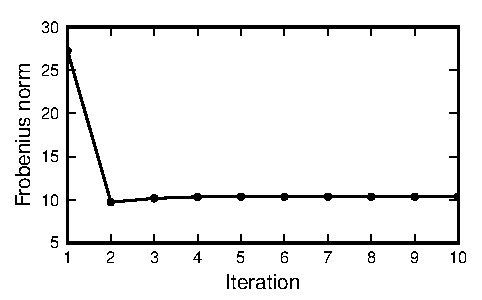
\includegraphics[scale=1]{./Graph/ConvergenceRate.pdf}
 		\caption{{\bf Convergence of the EM algorithm}. Representative plot of
the $\mathbf A(\boldsymbol\theta)$ Frobenius norm vs iterations of EM based algorithm. The change in the stopping criterion falls below $10^{-6}$ after less than 10 iterations.}
 	\label{fig:MRA-Convergence}
 \end{figure}     
% The spatial cutoff frequency of the observed field was used to specify the level of decomposition required to represent the field using the wavelets. Using an oversampling parameter of 5, the cutoff spatial frequency was $\nu_{cy} \approx 6.9 $ cycles/mm, obtained by averaging the spectral power of the spatial frequency (over time) from the observations \cite{Scerri2009}. Therefore, wavelets up to level $j=3$ (with the bandwidth $\approx[5,8]$ cycles/mm) can represent the significant spatial characteristics of the field, yielding $n_x = 131$ states. 


The actual connectivity kernel and the decomposition is plotted in Figure~\ref{fig:KernelEstimate}(a). No assumptions where made about the shape of the kernel. The reconstructed kernel is in good accordance with the actual kernel, where the actual kernel lies inside the confidence interval. The large standard deviation is due to the high number of parameters need to be estimated. The small error in the estimate is attributed to the MRA of the system used to form the estimator. Figure~\ref{fig:KernelEstimate}(b) and (c) illustrate the kernel scaling and wavelet functions, respectively. A total number of 25 basis functions was used to reconstruct the kernel, comprising 13 and 12 scaling and wavelet functions at $j=1$ accordingly. 
\begin{figure}[!t]
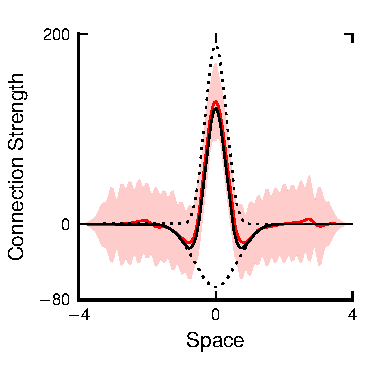
\includegraphics{./Graph/Figure5.pdf}
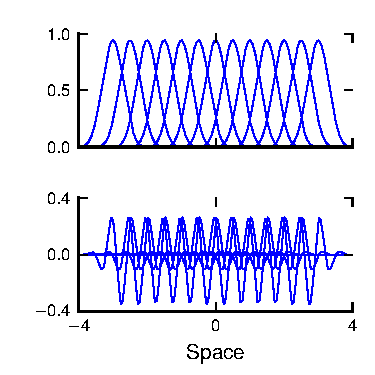
\includegraphics{./Graph/Figure6.pdf}
\caption{ {\bf Connectivity kernel estimate}. (\textbf{a}) The actual kernel and its components are shown by solid and dashed black lines, respectively. The mean kernel estimates over 200 realisations and confidence interval are shown by the red line and red shaded region ($\pm2$ std.). (\textbf{b}) Kernel scaling and wavelets functions, respectively, at $j=1$ used in the estimation algorithm.}
\label{fig:KernelEstimate}
\end{figure}

% \begin{figure}[!h] 
% 	\centering
% 		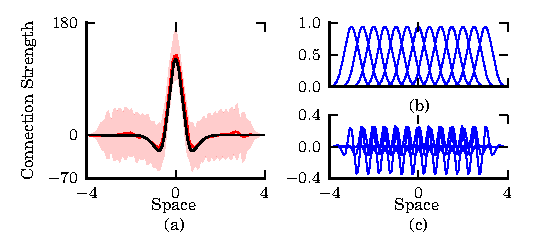
\includegraphics[scale=1]{./Graph/fig2.pdf}
% 		\caption{Connectivity kernel estimate. (a) The actual kernel and its components are shown by solid and dashed black lines, respectively. The mean kernel estimates over 200 realizations and confidence interval are shown by the red line and red shaded region ($\pm2$ std.). (b)-(c) Kernel scaling and wavelets functions, respectively, at $j=1$ used in estimation algorithm.}
% 	\label{fig:KernelEstimate}
% \end{figure}
 One snap shot of the field reconstruction, at different levels of approximation is given in Figures~\ref{fig:FieldEstimates100}, showing small discrepancy between the actual and estimated field at $j=3$. From this figure, it can be observed that the overall trend of the underlying field can be also captured at the coarser levels.
\begin{figure}[!t]
\centering
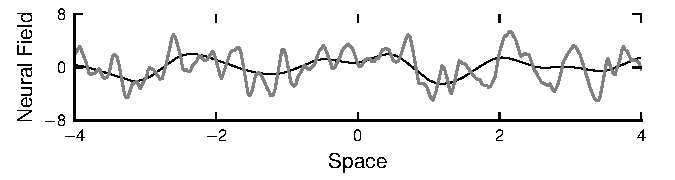
\includegraphics{./Graph/Figure4a.pdf}\\
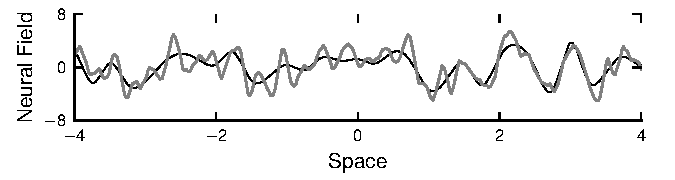
\includegraphics{./Graph/Figure4b.pdf}\\
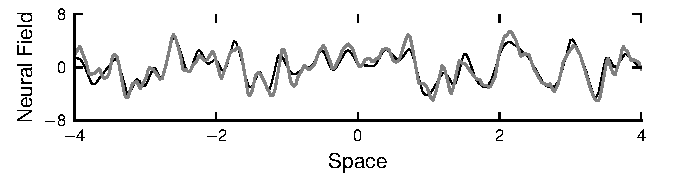
\includegraphics{./Graph/Figure4c.pdf}\\
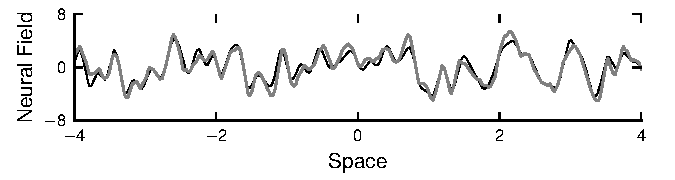
\includegraphics{./Graph/Figure4d.pdf}\\
\caption{ {\bf Examples of the actual and estimated neural fields for experiment I}. Actual (grey) and estimated (black) neural fields at a single time instant for different spatial resolutions. (\textbf{a}) $j=0$, $n_x=17$. (\textbf{b}) $j=1$, $n_x=33$. (\textbf{c}) $j=2$, $n_x=65$. (\textbf{d}) $j=3$, $n_x=131$.}
% (\textbf{e}) $j=4$, $n_x=263$.
\label{fig:FieldEstimates100}
\end{figure}
\begin{figure}[t]
	\centering
		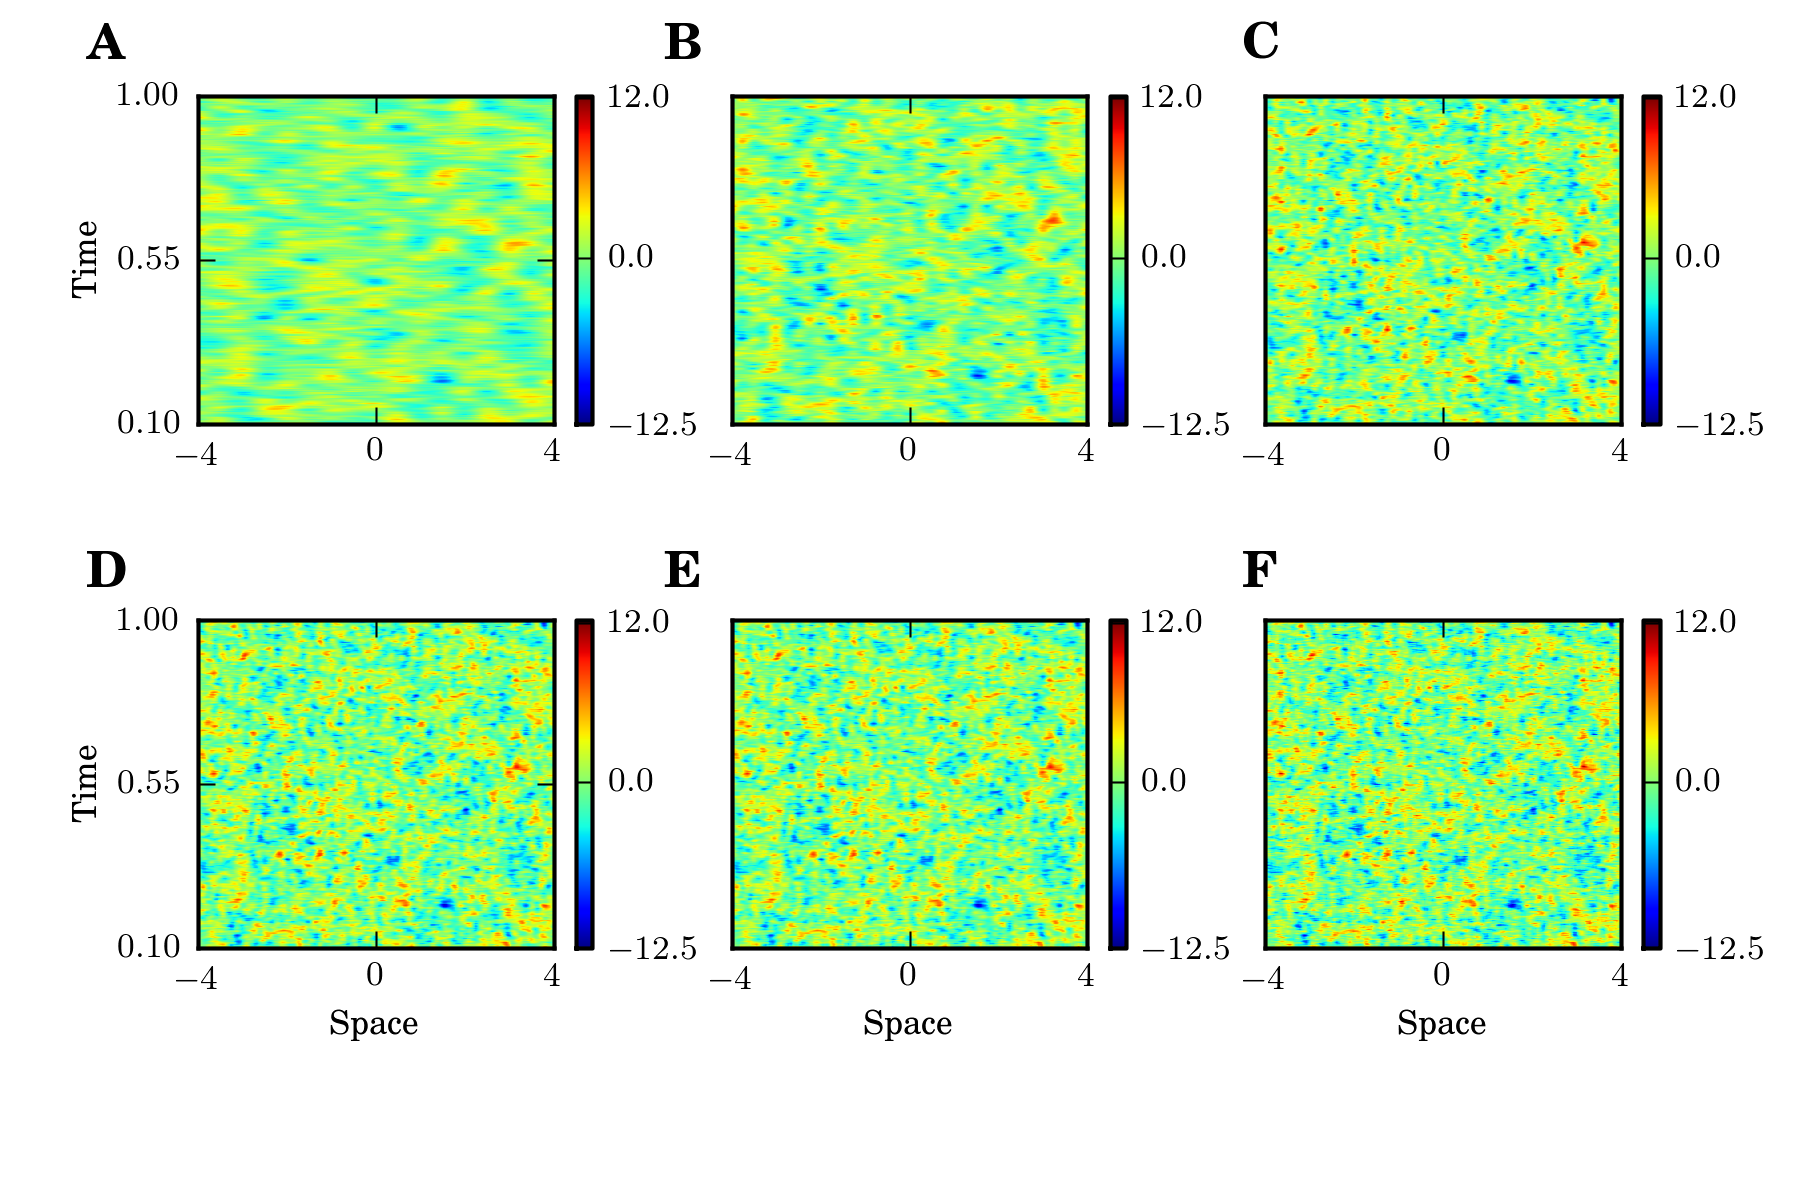
\includegraphics[scale=1]{./Graph/STMultiRes.png}
	\caption{{\bf Actual and estimated spatiotemporal neural field at different spatial resolutions}. (\textbf{A}) The reconstructed field of the reduced model using at $j=0$. (\textbf{B}) The reconstructed field at $j=1$. (\textbf{C}) The reconstructed field at $j=2$. (\textbf{D}) The reconstructed field at $j=3$. (\textbf{E}) The reconstructed at $j=4$. (\textbf{F}) The actual field.}
	\label{fig:FieldEstimation}
\end{figure}

\subsection{Experiment II}
To study the performance of different models with various MRA capabilities, a single realisation was obtained using \eqref{eq:DiscreteTimeModel} and \eqref{eq:ObservationEquation} under the same circumstances of the previous experiment. The generated data set was then employed to estimate the underlying field and the connectivity kernel parameters using different state-space models, $j=0$ up to $j=4$. The RMSE of the field estimation at different levels of approximation is shown in Figure~\ref{fig:RMSE}. By increasing the value of $j$, error in the estimation decreases and converges to a steady value of 0.71, confirming that $j=3$ is in fact adequate to capture the dynamics of the underlying field. The estimated field at a single time instant is shown in Figure~\ref{fig:FieldEstimates200}. The experiment was performed several times and the results were consistent over each run.
 \begin{figure}[!t] 
 	\centering
 		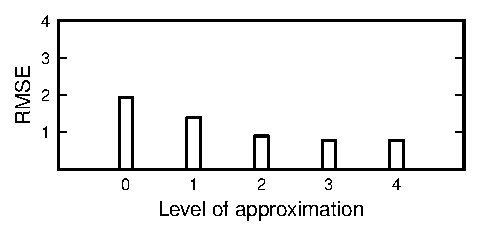
\includegraphics[scale=1]{./Graph/Figure3.pdf}
 		\caption{{\bf Error in the field reconstruction for experiment II}. MRMSE of the estimated field of models with different level of approximations. $j=0$, $RMSE = 1.83$; $j=1$, $RMSE = 1.41$; $j=2$, $RMSE = 0.83$; $j=3$, $RMSE = 0.71$; $j=4$, $RMSE=0.71$}
 	\label{fig:RMSE}
 \end{figure} 
\begin{figure}[!t]
\centering
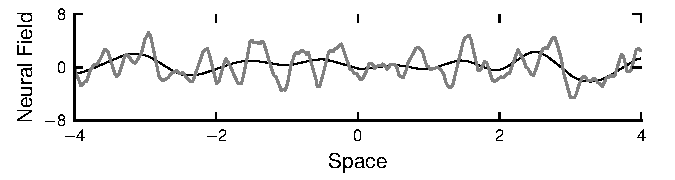
\includegraphics{./Graph/Figure5a.pdf}\\
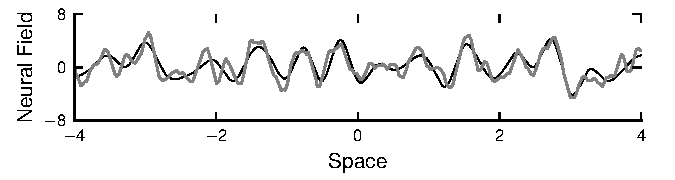
\includegraphics{./Graph/Figure5b.pdf}\\
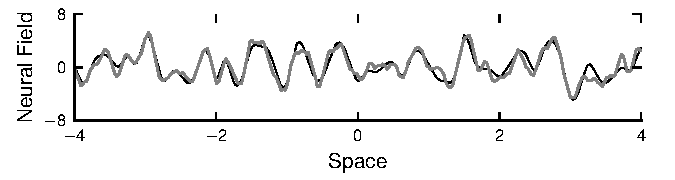
\includegraphics{./Graph/Figure5c.pdf}\\
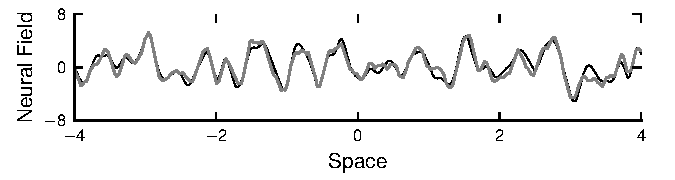
\includegraphics{./Graph/Figure5d.pdf}\\
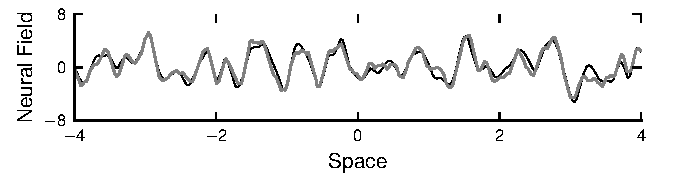
\includegraphics{./Graph/Figure5e.pdf}\\
\caption{ {\bf Examples of the actual and estimated neural fields for experiment II}. Actual (grey) and estimated (black) neural fields at a single time instant  for models with different spatial resolutions. (\textbf{a}) $j=0$, $n_x=17$. (\textbf{b}) $j=1$, $n_x=33$. (\textbf{c}) $j=2$, $n_x=65$. (\textbf{d}) $j=3$, $n_x=131$. (\textbf{e}) $j=4$, $n_x=263$.}
\label{fig:FieldEstimates200}
\end{figure}
% The field reconstruction, at different levels of approximations, is shown in \figurename{\ref{fig:FieldEstimates}}. The figure confirms that $j=3$ is adequate to capture the dynamics of the underlying field, where the RMSE converges to a steady value of 0.78. Fig.~\ref{fig:FieldEstimates} confirms good state estimation performance, where the estimated field is in good accordance with the true field. 
% \begin{figure}[!h] 
% 	\centering
% 		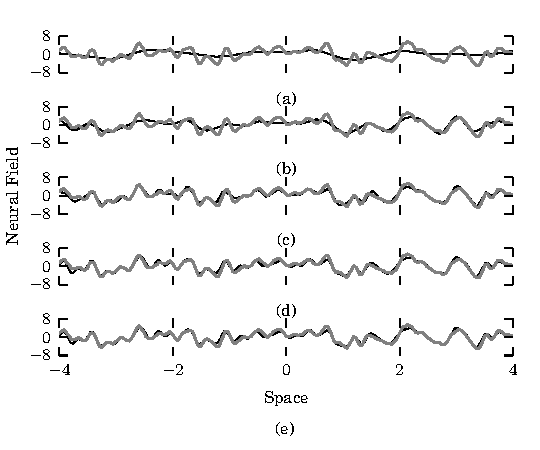
\includegraphics[scale=1]{./Graph/fig1.pdf}
% 		\caption{Actual (gray) and estimated (black) neural fields at a time instant for different spatial resolutions. (a) $j=0$, $n_x=17$, $RMSE = 1.93$. (b) $j=1$, $n_x=33$, $RMSE = 1.39$. (c) $j=2$, $n_x=65$, $RMSE = 0.90$. (d) $j=3$, $n_x=131$, $RMSE = 0.78$. (e) $j=4$, $n_x=263$, $RMSE=0.78$.}
% 	\label{fig:FieldEstimates}
% \end{figure} 

% \caption{The actual connectivity kernel is shown with the black solid line. The estimated kernel and confidence interval is shown by the red line and red shaded region ($\pm2$ std.). The 7 weighted kernel basis functions are shown by the black dashed lines.}
\section{Discussion}
In this paper, we have presented a novel model-based framework for estimating cortical dynamics from electrophysiological measurements. The novel and key developments of the paper include the multi-resolution FEM representation of the neural field, and the estimator for an intracortical connectivity kernel with an arbitrary shape. This work is significant, as the ability to create patient specific neural field models has the potential to contribute to our understanding and improve treatment of diseases resulting from abnormal neurodynamics, such as epilepsy. Other groups have previously highlighted the importance of a multi-resolution approach in neural field modeling. It is thought that the dynamics and connectivity structure differs at different spatial scales~\citep{Qubbaj2009,Breakspear2005}. %\dean{This is a test to see if we can fit something about Breaky's paper in here. It would be nice to slot something in here because he used wavelets.} 

For a larger space or in a case where the connectivity kernel decomposition comprises of  many scale levels, the number of parameters to be estimated increases significantly. One solution to this problem could be expectation-conditional maximisation (ECM) \citep{Meng1993,Meng1994} which replaces the M-step by a series of computationally simplified conditional maximization (CM) steps. The ECM is a class of generalised EM (GEM)  algorithms in which the $\mathcal{Q}$-function is increased rather than being maximised \citep{Fessler1994}. 

For systems with a high number of states, the ensemble Kalman smoother (EnKS) \citep{Evensen2003,Evensen2009a,Evensen2009} provides an alternative to the RTS smoother used in this work. The EnKS is a sequential Monte Carlo (MC) method where the state covariance matrix is approximated by a large stochastic ensemble of model states, thus alleviating computational load due to the storage and forward integration of the state covariance matrix. However, combining the EnKS with the EM algorithm suffers from the loss of monotonicity property --- increase in the likelihood function--- as MC error will be introduced at the E-step.

Typically, a sequence of likelihood values will converge to a stationary point i.e. global (local) maximum or a saddle point. If the sequence of the EM is trapped in a local maximum or a saddle point, a small random perturbation diverges the algorithm from such stationary values \citep{McLachlan1997}. In general, convergence of the EM algorithm to any stationary point depends on the initialisation. In the examples presented in this paper, a bounded sequence of the state vectors was used to initialise the algorithm, which gave a satisfactory convergence and good state and parameter estimations.


The MRAIDE approach is not limited to neural fields; the framework can be applied to modeling other multi-resolution spatiotemporal dynamical systems such as weather systems, ecological systems, and others~\citep{Wikle2002,Xu2005}. 
% \ken{meteorology [76, 88, 94, 222, 232], epidemiology [123, 137, 218], physics [32, 85, 129, 231], environmental science [45, 87, 183, 204] and economics [31, 48, 165]. (This is copy and paste from my thesis ... parham I'll get you the references later)}. \parham{Mike,Ken: can add to this list?}\mike{While I love this kind of thing for a review, I'm not sure we have space for this kind of thing? Also it's not terribly specific. I think it's better to stick to how it has the potential to model brains in a manner that rocks, rather than loosely saying it could be applied to any spatiotemporal system, i.e. literally everything.}

  % \mike{The framework makes two key assumptions about the cortex: a linear activation function and stationary dynamics. Our main aim for this framework in the future is to relax these assumptions using the multi-resolution decomposition. While the decomposition itself holds, efficiently performing nonlinear smoothing in the much larger state space remains a challenge. Additional avenues for future work include extending the model to capture a second order synaptic response kernel, and time delays \parham{at lower spatial resolutions}.  The estimation techniques should also be extended to deal with spatial and temporal heterogeneity in the kernel. Finally, the majority of our current work involves applying this framework to collected data, primarily for the use of seizure detection and mitigation.}

% In order to apply the framework to real data some assumptions must be made. A critical assumption is that the model provides an apt description of the cortical dynamics.

To demonstrate MRAIDE framework, an assumption was made where the firing rate behaves linearly. The implementation of the framework in the non-linear case can be addressed as future work. Another future avenue would be the modification of the estimation framework to perform efficiently at higher dimensions. The reconstruction of the neural field requires $2^n-1$ wavelets, where $n$ is the dimension of the space. For example a two-dimensional MRA can be implemented using 2-D scaling and wavelet functions built up using the tensor-product approach \citep{Meyer1992}. In this case three wavelet functions are required to  extract fine features of the field at vertical, horizontal and diagonal orientations. Although provided formulations can be easily extended into two dimensions the  computational load of the estimation algorithm will be significant. It is important to investigate methods for choosing basis functions to balance the complexity with the reconstruction capability of the model.
 
The authors acknowledge that there is, and will always be, a discrepancy between the model and cortex. Nevertheless, the model-based framework proposed in this paper may enable meaningful state tracking and connectivity estimation. The key development is the multi-resolution decomposition forming the state-space model. While the decomposition holds for more sophisticated models, efficiently performing nonlinear smoothing in the large state-space remains a challenge. 

Additional extension for future work include extending the model to capture a second order synaptic response kernel, The second order postsynaptic kernel proposed in \citet{VanRotterdam1982} leads to dynamics that are more reminiscent to real postsynaptic potentials. 

Another extension of this framework is the inclusion of finite distant-dependent action potential propagation velocity into the parametric neural field equations. In small networks the delays via propagation can be neglected, however they must be accounted for in large scale networks. For instance, it is shown by \citet{Ghosh2008} that inclusion of time delays arising from propagation along connecting fibres are essential for the fluctuations to be appeared in the default networks. Finally, future work should be directed towards applying and validating the framework on real data.

\section{Appendix}
\subsection{Inner product of two B-spline scaling functions}\label{ap:InnerProductOfBsplines}
In this section, an analytic formula is derived for the inner product of two B-spline scaling functions. Consider two B-spline scaling functions of order $m$ and $m'$. The support of $N_m\left(s\right)$ is $\left[ 0,m\right]$ and  is symmetric with respect to $r=\frac{m}{2}$, i.e.
\begin{align}\label{eq:APP-SymmetrySplieEq}
 N_{m}\left(\frac{m}{2}+r\right)=N_{m}\left(\frac{m}{2}-r\right).
\end{align}
A direct consequence of \eqref{eq:APP-SymmetrySplieEq} is 
\begin{align}
 N_{m}\left(r\right)=N_{m}\left(m-r\right).
\end{align}
Therefore
\begin{align}
\int_{-\infty}^{+\infty}N_{m}\left(r-l_{1}\right)N_{m'}\left(r-l_{2}\right)ds&=\int_{-\infty}^{+\infty}N_{m}\left(m-r+l_{1}\right)N_{m'}\left(r-l_{2}\right)dr \nonumber \\
&=\int_{-\infty}^{+\infty}N_{m}\left(m+l_{1}-l_{2}-u\right)N_{m'}\left(u\right)du \nonumber \\
&=\left(N_m \ast N_{m'}\right) \left(m+l_{1}-l_{2}\right) \nonumber \\
&=N_{m+m'}\left(m+l_{1}-l_{2}\right) \nonumber \\
&=N_{m+m'}\left(m'+l_{2}-l_{1}\right).
\end{align}
\subsection{Induction}\label{ap:Induction}
For $n_1$ in equation \eqref{eq:MRA-ConvertingFormulaForscalingFunctions} we have
\begin{align}
 N_{m}\left(r\right)&=\sum_{n_1=0}^{m} \left[\mathbf p\right]_{n_1} N_{m}\left(2r-n_1\right) \label{eq:App-TwoScalepair1},
  \end{align}
which clearly holds (see \eqref{eq:MRA-TwoScalepair1}). Now assuming \eqref{eq:MRA-ConvertingFormulaForscalingFunctions} for $n_{j-1}$ we have
\begin{align}\label{eq:app-ConvertingFormulaForscalingFunctions}
 &N_m(r)=\nonumber \\
&\sum_{n_1,n_2, \dots n_{j-1}=0}^{m}\left[\mathbf p\right]_{n_1} \left[\mathbf p\right]_{n_2}\dots \left[\mathbf p\right]_{n_{j-1}}N_m(2^{j-1}r-k_{n_1,n_2, \dots, n_{j-1}}),
\end{align}
$N_m(2^{j-1}r-k_{n_1,n_2, \dots, n_{j-1}})$ can be written in terms of $N_m(2^{j}r)$ as
\begin{align}\label{eq:AppendixNj-1intermsofNj}
 &N_m(2^{j-1}r-k_{n_1,n_2, \dots, n_{j-1}})=\nonumber \\
&\sum_{n_j=0}^m \left[\mathbf p\right]_{n_j}N_m(2^jr-2\times k_{n_1,n_2, \dots, n_{j-1}}-n_j)\nonumber \\
&=\sum_{n_j=0}^m \left[\mathbf p\right]_{n_j}N_m(2^jr- k_{n_1,n_2, \dots, n_{j}})
\end{align}
Substituting \eqref{eq:AppendixNj-1intermsofNj} in to \eqref{eq:MRA-ConvertingFormulaForscalingFunctions} completes the proof. 

\subsection{Lower bound on likelihood function}\label{ap:Lowerbound}
A derivation of the lower bound on the likelihood function that is based on \citet{Bishop2006} is provided in this Appendix. We want to maximise the likelihood function which is difficult to perform directly
\begin{equation}
 p(\mathbf Y;\boldsymbol\theta)=\int_{\mathbf X}p(\mathbf X,\mathbf Y;\boldsymbol\theta)d\mathbf X.
\end{equation}   
Maximising the likelihood in terms of the parameter set is equivalent to the log-likelihood maximisation, as both the likelihood and log-likelihood functions share the same maximiser due to the monotonicity of the logarithm function. For any choice of distribution defined over the latent variables, $q(\mathbf X)$, the following decomposition holds
\begin{equation}\label{eq:EM-loglikelihooddecomposition}
 \ln~p(\mathbf Y;\boldsymbol\theta)=\mathcal{L}(q,\boldsymbol\theta)+\mathrm{KL}(q\parallel p),
\end{equation}
where
\begin{align}
 \mathcal{L}(q,\boldsymbol\theta)&=\int_{\mathbf X} q(\mathbf X)\ln\left\lbrace \frac{p(\mathbf X,\mathbf Y;\boldsymbol\theta)}{q(\mathbf X)} \right\rbrace d\mathbf X \label{eq:EM-decomposition1}\\
\mathrm{KL}(q\parallel p)&=-\int_{\mathbf X}q(\mathbf X)\ln\left\lbrace \frac{p(\mathbf X \mid \mathbf Y;\boldsymbol\theta)}{q(\mathbf X)} \right\rbrace d\mathbf X. \label{eq:EM-decomposition2}
\end{align}
Equation \eqref{eq:EM-loglikelihooddecomposition} can be verified by applying the probability product rule to the joint distribution $p(\mathbf X,\mathbf Y;\boldsymbol\theta)$ in \eqref{eq:EM-decomposition1} giving
\begin{align}
	\mathcal{L}(q,\boldsymbol\theta)+\mathrm{KL}(q\parallel p)&= \int_{\mathbf X} q(\mathbf X)\ln\left\lbrace \frac{p(\mathbf X \mid \mathbf Y;\boldsymbol\theta)p(\mathbf Y;\boldsymbol\theta)}{q(\mathbf X)} \right\rbrace d\mathbf X \nonumber\\
	&- \int_{\mathbf X}q(\mathbf X)\ln\left\lbrace \frac{p(\mathbf X \mid \mathbf Y;\boldsymbol\theta)}{q(\mathbf X)} \right\rbrace d\mathbf X\nonumber\\
	&= \int_{\mathbf X}q(\mathbf X)\ln p(\mathbf Y; \boldsymbol\theta)d\mathbf X.
\end{align}
Noting  $q(\mathbf X)$ is a normalised distribution that integrates to one gives the log-likelihood function. Note \eqref{eq:EM-decomposition2} is the Kullback-Liebler distance between distributions $p(\mathbf X \mid \mathbf Y;\boldsymbol\theta)$ and $q(\mathbf X)$, therefore,
\begin{equation}
	\mathrm{KL}(q\parallel p)\ge 0.
\end{equation}   
The equality holds if and only if $q(\mathbf X)=p(\mathbf X \mid \mathbf Y;\boldsymbol\theta)$. It follows from equation \eqref{eq:EM-loglikelihooddecomposition}, that the quantity $\mathcal{L}(q,\boldsymbol\theta)$ is a lower bound on the log-likelihood function, i.e.
\begin{equation}
 \mathcal{L}(q,\boldsymbol\theta)\le \ln~p(\mathbf Y\mid\boldsymbol\theta)
	\end{equation} 

The EM algorithm alternates between maximising the lower bound with respect to the distribution $q(\mathbf X)$ and the parameter set $\boldsymbol\theta$, respectively, while holding the other fixed. Suppose that the current estimate of the parameter set is $\boldsymbol\theta'$, in the E-step the lower bound is maximised with respect to the distribution $q(\mathbf X)$ while $\boldsymbol\theta'$ is fixed. Since the value of $p(\mathbf Y;\boldsymbol\theta')$ is independent of $q(\mathbf X)$ the maximum of the lower bound occurs when the KL distance disappears or in other words when $q(\mathbf X)$ is exactly the conditional distribution $p(\mathbf X \mid \mathbf Y;\boldsymbol\theta)$. At this point, the lower bound becomes equal to the log-likelihood function. Note in the state-space model the E-step is equivalent to the smoothing problem. The maximum in the M-step is obtained by maximising the lower bound with respect to the parameter set while the distribution $q(\mathbf X)$ is held fixed. Since the distribution $q(\mathbf X)$ is computed using the old parameter estimates and kept fixed during the M-step, it is not equal to $p(\mathbf X \mid \mathbf Y;\boldsymbol\theta)$, resulting in a non-zero KL distance. Therefore, the growth of the log-likelihood function is greater than the growth of the lower bound. Substituting $p(\mathbf X \mid \mathbf Y;\boldsymbol\theta')$ for $q(\mathbf X)$ in \eqref{eq:EM-decomposition1} gives
\begin{align}
 \mathcal{L}(q,\boldsymbol\theta)&=\int_{\mathbf X} p(\mathbf X\mid\mathbf Y;\boldsymbol\theta')\ln p(\mathbf X,\mathbf Y;\boldsymbol\theta)~d\mathbf X-\int_{\mathbf X} p(\mathbf X\mid\mathbf Y;\boldsymbol\theta')\ln p(\mathbf X\mid\mathbf Y;\boldsymbol\theta')~d\mathbf X \nonumber \\
&= \mathbf E_{\boldsymbol\theta'}\left[ \ln p(\mathbf X,\mathbf Y;\boldsymbol\theta)\right] +\mathrm{const.}\nonumber\\
&=\mathcal{Q}(\boldsymbol\theta,\boldsymbol\theta')+\mathrm{const.}~,\label{eq:EM-ComDaLogLike}
\end{align}
where $ \mathbf E_{\boldsymbol \theta'}\left[ \cdot\right] $ denotes expectation taken with respect to the marginal distribution of the states conditioned on the observed field and the current estimate of the parameter set, i.e.  $p(\mathbf X\mid\mathbf Y;\boldsymbol \theta'$). The constant term is the negative entropy of $q(\mathbf X)$ and is independent of $\boldsymbol\theta$.   It becomes clear from \eqref{eq:EM-ComDaLogLike} that, the M-step essentially maximises the expectation of the complete data log-likelihood. 
\section{Calculation of $\boldsymbol\Xi_{0}$ and $\boldsymbol\Xi_{1}$}\label{ap:Xiderivation}
The expressions for $\boldsymbol\Xi_{0}$ and $\boldsymbol\Xi_{1}$ in terms of smoother outputs can be found in \cite{Shumway2000}, here we present the derivation for completeness.  The expression for  $\boldsymbol\Xi_{0}$ as defined in equation~\eqref{eq:Xi0} of the main text is given by
   \begin{equation}\label{eq:appXi0}
	 \boldsymbol\Xi_0=\mathbf E_{\theta'}\left[\sum_{t=0}^{T-1}\mathbf x_t\mathbf x_{t+1}^\top\right].
	\end{equation}                                                                                                
	We start by expanding the equation \eqref{eq:appXi0}, giving
	
\begin{align}\label{eq:Xi0derivation0} 
 \mathbf M_{t+1}&=\mathbf E_{\theta'}\left[(\mathbf x_t-\mathbf{\hat x}_t)(\mathbf x_{t+1}-\mathbf{\hat x}_{t+1})^\top\right] \nonumber \\
&=\mathbf E_{\theta'}\left[\mathbf x_t\mathbf x_{t+1}^\top\right]-\mathbf E_{\theta'}\left[\mathbf x_t\hat{\mathbf x}_{t+1}^\top\right]-\mathbf E_{\theta'}\left[\hat{\mathbf x}_t\mathbf x_{t+1}^\top\right]+\mathbf E_{\theta'}\left[\hat{\mathbf x}_t\hat{\mathbf x}_{t+1}^\top\right]  \nonumber \\
&= \mathbf E_{\theta'}\left[\mathbf x_t\mathbf x_{t+1}^\top\right]-\hat{\mathbf x}_t\hat{\mathbf x}_{t+1}^\top-\hat{\mathbf x}_t\hat{\mathbf x}_{t+1}^\top+\hat{\mathbf x}_t\hat{\mathbf x}_{t+1}^\top\nonumber \\
&= \mathbf E_{\theta'}\left[\mathbf x_t\mathbf x_{t+1}^\top\right]-\hat{\mathbf x}_t\hat{\mathbf x}_{t+1}^\top.
\end{align}
Rearranging  equation \eqref{eq:Xi0derivation0} we get
\begin{equation}\label{eq:Xi0derivation1}
 \mathbf E_{\theta'}\left[\mathbf x_t\mathbf x_{t+1}^\top\right]=\mathbf M_{t+1}+\mathbf {\hat x}_t\mathbf{\hat x}_{t+1}^\top
\end{equation}
substituting \ref{eq:Xi0derivation1} into \ref{eq:appXi0}, noting the expectation commutes with the sum we get
\begin{equation}
 \boldsymbol\Xi_1=\sum_{t=0}^{T-1}\left(\mathbf M_{t+1}+\mathbf{\hat x}_t\mathbf{\hat x}_{t+1}^\top\right)
\end{equation}   
An expression for $\boldsymbol\Xi_1$ in terms of the smoothed states can be also found in a similar way by expanding the covariance matrix,
\begin{equation}\label{eq:appXi1}
 \boldsymbol\Xi_1=\mathbf E_{\theta'}\left[\sum_{t=0}^{T-1}\mathbf x_{t}\mathbf x_{t}^\top\right],
\end{equation}
therefore we can write
\begin{equation}\label{eq:Xi1derivation1}
 \mathbf E_{\theta'}\left[\mathbf x_{t}\mathbf x_{t}^\top\right]=\mathbf P_{t}+\mathbf {\hat x}_{t}\mathbf{\hat x}_{t}^\top,
\end{equation}
substituting \ref{eq:Xi1derivation1} into \ref{eq:appXi1} we get
\begin{equation}
 \boldsymbol\Xi_1=\sum_{t=0}^{T-1}\left(\mathbf P_{t}+\mathbf{\hat x}_{t}\mathbf{\hat x}_{t}^\top\right).
\end{equation}
\ifCLASSOPTIONcaptionsoff
  \newpage
\fi

%   \newpage
% \bibliographystyle{unsrt} 
\bibliographystyle{apalike}
\bibliography{MRAIDE}

% \bibliographystyle{IEEEtran}
% argument is your BibTeX string definitions and bibliography database(s)
 % \bibliography{IEEEabrv,MRAIDE}


\end{document}


